\documentclass[1p]{elsarticle_modified}
%\bibliographystyle{elsarticle-num}

%\usepackage[colorlinks]{hyperref}
%\usepackage{abbrmath_seonhwa} %\Abb, \Ascr, \Acal ,\Abf, \Afrak
\usepackage{amsfonts}
\usepackage{amssymb}
\usepackage{amsmath}
\usepackage{amsthm}
\usepackage{scalefnt}
\usepackage{amsbsy}
\usepackage{kotex}
\usepackage{caption}
\usepackage{subfig}
\usepackage{color}
\usepackage{graphicx}
\usepackage{xcolor} %% white, black, red, green, blue, cyan, magenta, yellow
\usepackage{float}
\usepackage{setspace}
\usepackage{hyperref}

\usepackage{tikz}
\usetikzlibrary{arrows}

\usepackage{multirow}
\usepackage{array} % fixed length table
\usepackage{hhline}

%%%%%%%%%%%%%%%%%%%%%
\makeatletter
\renewcommand*\env@matrix[1][\arraystretch]{%
	\edef\arraystretch{#1}%
	\hskip -\arraycolsep
	\let\@ifnextchar\new@ifnextchar
	\array{*\c@MaxMatrixCols c}}
\makeatother %https://tex.stackexchange.com/questions/14071/how-can-i-increase-the-line-spacing-in-a-matrix
%%%%%%%%%%%%%%%

\usepackage[normalem]{ulem}

\newcommand{\msout}[1]{\ifmmode\text{\sout{\ensuremath{#1}}}\else\sout{#1}\fi}
%SOURCE: \msout is \stkout macro in https://tex.stackexchange.com/questions/20609/strikeout-in-math-mode

\newcommand{\cancel}[1]{
	\ifmmode
	{\color{red}\msout{#1}}
	\else
	{\color{red}\sout{#1}}
	\fi
}

\newcommand{\add}[1]{
	{\color{blue}\uwave{#1}}
}

\newcommand{\replace}[2]{
	\ifmmode
	{\color{red}\msout{#1}}{\color{blue}\uwave{#2}}
	\else
	{\color{red}\sout{#1}}{\color{blue}\uwave{#2}}
	\fi
}

\newcommand{\Sol}{\mathcal{S}} %segment
\newcommand{\D}{D} %diagram
\newcommand{\A}{\mathcal{A}} %arc


%%%%%%%%%%%%%%%%%%%%%%%%%%%%%5 test

\def\sl{\operatorname{\textup{SL}}(2,\Cbb)}
\def\psl{\operatorname{\textup{PSL}}(2,\Cbb)}
\def\quan{\mkern 1mu \triangleright \mkern 1mu}

\theoremstyle{definition}
\newtheorem{thm}{Theorem}[section]
\newtheorem{prop}[thm]{Proposition}
\newtheorem{lem}[thm]{Lemma}
\newtheorem{ques}[thm]{Question}
\newtheorem{cor}[thm]{Corollary}
\newtheorem{defn}[thm]{Definition}
\newtheorem{exam}[thm]{Example}
\newtheorem{rmk}[thm]{Remark}
\newtheorem{alg}[thm]{Algorithm}

\newcommand{\I}{\sqrt{-1}}
\begin{document}

%\begin{frontmatter}
%
%\title{Boundary parabolic representations of knots up to 8 crossings}
%
%%% Group authors per affiliation:
%\author{Yunhi Cho} 
%\address{Department of Mathematics, University of Seoul, Seoul, Korea}
%\ead{yhcho@uos.ac.kr}
%
%
%\author{Seonhwa Kim} %\fnref{s_kim}}
%\address{Center for Geometry and Physics, Institute for Basic Science, Pohang, 37673, Korea}
%\ead{ryeona17@ibs.re.kr}
%
%\author{Hyuk Kim}
%\address{Department of Mathematical Sciences, Seoul National University, Seoul 08826, Korea}
%\ead{hyukkim@snu.ac.kr}
%
%\author{Seokbeom Yoon}
%\address{Department of Mathematical Sciences, Seoul National University, Seoul, 08826,  Korea}
%\ead{sbyoon15@snu.ac.kr}
%
%\begin{abstract}
%We find all boundary parabolic representation of knots up to 8 crossings.
%
%\end{abstract}
%\begin{keyword}
%    \MSC[2010] 57M25 
%\end{keyword}
%
%\end{frontmatter}

%\linenumbers
%\tableofcontents
%
\newcommand\colored[1]{\textcolor{white}{\rule[-0.35ex]{0.8em}{1.4ex}}\kern-0.8em\color{red} #1}%
%\newcommand\colored[1]{\textcolor{white}{ #1}\kern-2.17ex	\textcolor{white}{ #1}\kern-1.81ex	\textcolor{white}{ #1}\kern-2.15ex\color{red}#1	}

{\Large $\underline{12a_{0888}~(K12a_{0888})}$}

\setlength{\tabcolsep}{10pt}
\renewcommand{\arraystretch}{1.6}
\vspace{1cm}\begin{tabular}{m{100pt}>{\centering\arraybackslash}m{274pt}}
\multirow{5}{120pt}{
	\centering
	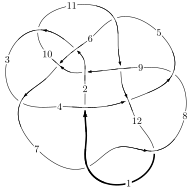
\includegraphics[width=112pt]{../../../GIT/diagram.site/Diagrams/png/1689_12a_0888.png}\\
\ \ \ A knot diagram\footnotemark}&
\allowdisplaybreaks
\textbf{Linearized knot diagam} \\
\cline{2-2}
 &
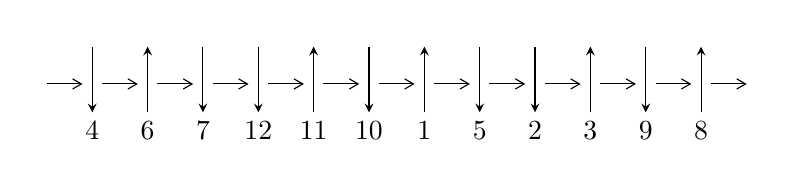
\begin{tikzpicture}[x=20pt, y=17pt]
	% nodes
	\node (C0) at (0, 0) {};
	\node (C1) at (1, 0) {};
	\node (C1U) at (1, +1) {};
	\node (C1D) at (1, -1) {4};

	\node (C2) at (2, 0) {};
	\node (C2U) at (2, +1) {};
	\node (C2D) at (2, -1) {6};

	\node (C3) at (3, 0) {};
	\node (C3U) at (3, +1) {};
	\node (C3D) at (3, -1) {7};

	\node (C4) at (4, 0) {};
	\node (C4U) at (4, +1) {};
	\node (C4D) at (4, -1) {12};

	\node (C5) at (5, 0) {};
	\node (C5U) at (5, +1) {};
	\node (C5D) at (5, -1) {11};

	\node (C6) at (6, 0) {};
	\node (C6U) at (6, +1) {};
	\node (C6D) at (6, -1) {10};

	\node (C7) at (7, 0) {};
	\node (C7U) at (7, +1) {};
	\node (C7D) at (7, -1) {1};

	\node (C8) at (8, 0) {};
	\node (C8U) at (8, +1) {};
	\node (C8D) at (8, -1) {5};

	\node (C9) at (9, 0) {};
	\node (C9U) at (9, +1) {};
	\node (C9D) at (9, -1) {2};

	\node (C10) at (10, 0) {};
	\node (C10U) at (10, +1) {};
	\node (C10D) at (10, -1) {3};

	\node (C11) at (11, 0) {};
	\node (C11U) at (11, +1) {};
	\node (C11D) at (11, -1) {9};

	\node (C12) at (12, 0) {};
	\node (C12U) at (12, +1) {};
	\node (C12D) at (12, -1) {8};
	\node (C13) at (13, 0) {};

	% arrows
	\draw[->,>={angle 60}]
	(C0) edge (C1) (C1) edge (C2) (C2) edge (C3) (C3) edge (C4) (C4) edge (C5) (C5) edge (C6) (C6) edge (C7) (C7) edge (C8) (C8) edge (C9) (C9) edge (C10) (C10) edge (C11) (C11) edge (C12) (C12) edge (C13) ;	\draw[->,>=stealth]
	(C1U) edge (C1D) (C2D) edge (C2U) (C3U) edge (C3D) (C4U) edge (C4D) (C5D) edge (C5U) (C6U) edge (C6D) (C7D) edge (C7U) (C8U) edge (C8D) (C9U) edge (C9D) (C10D) edge (C10U) (C11U) edge (C11D) (C12D) edge (C12U) ;
	\end{tikzpicture} \\
\hhline{~~} \\& 
\textbf{Solving Sequence} \\ \cline{2-2} 
 &
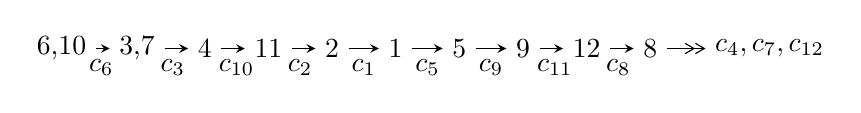
\begin{tikzpicture}[x=23pt, y=7pt]
	% node
	\node (A0) at (-1/8, 0) {6,10};
	\node (A1) at (17/16, 0) {3,7};
	\node (A2) at (17/8, 0) {4};
	\node (A3) at (25/8, 0) {11};
	\node (A4) at (33/8, 0) {2};
	\node (A5) at (41/8, 0) {1};
	\node (A6) at (49/8, 0) {5};
	\node (A7) at (57/8, 0) {9};
	\node (A8) at (65/8, 0) {12};
	\node (A9) at (73/8, 0) {8};
	\node (C1) at (1/2, -1) {$c_{6}$};
	\node (C2) at (13/8, -1) {$c_{3}$};
	\node (C3) at (21/8, -1) {$c_{10}$};
	\node (C4) at (29/8, -1) {$c_{2}$};
	\node (C5) at (37/8, -1) {$c_{1}$};
	\node (C6) at (45/8, -1) {$c_{5}$};
	\node (C7) at (53/8, -1) {$c_{9}$};
	\node (C8) at (61/8, -1) {$c_{11}$};
	\node (C9) at (69/8, -1) {$c_{8}$};
	\node (A10) at (11, 0) {$c_{4},c_{7},c_{12}$};

	% edge
	\draw[->,>=stealth]	
	(A0) edge (A1) (A1) edge (A2) (A2) edge (A3) (A3) edge (A4) (A4) edge (A5) (A5) edge (A6) (A6) edge (A7) (A7) edge (A8) (A8) edge (A9) ;
	\draw[->>,>={angle 60}]	
	(A9) edge (A10);
\end{tikzpicture} \\ 

\end{tabular} \\

\footnotetext{
The image of knot diagram is generated by the software ``\textbf{Draw programme}" developed by Andrew Bartholomew(\url{http://www.layer8.co.uk/maths/draw/index.htm\#Running-draw}), where we modified some parts for our purpose(\url{https://github.com/CATsTAILs/LinksPainter}).
}\phantom \\ \newline 
\centering \textbf{Ideals for irreducible components\footnotemark of $X_{\text{par}}$} 
 
\begin{align*}
I^u_{1}&=\langle 
6.54150\times10^{2113} u^{198}+2.25876\times10^{2114} u^{197}+\cdots+8.55458\times10^{2111} b-4.60399\times10^{2114},\\
\phantom{I^u_{1}}&\phantom{= \langle  }6.83826\times10^{2112} u^{198}+2.36400\times10^{2113} u^{197}+\cdots+2.94986\times10^{2110} a-4.90075\times10^{2113},\\
\phantom{I^u_{1}}&\phantom{= \langle  }u^{199}+4 u^{198}+\cdots+109 u-4\rangle \\
I^u_{2}&=\langle 
6.56727\times10^{107} u^{47}+2.94736\times10^{108} u^{46}+\cdots+2.61573\times10^{107} b+7.33724\times10^{107},\\
\phantom{I^u_{2}}&\phantom{= \langle  }2.23775\times10^{108} u^{47}+1.01685\times10^{109} u^{46}+\cdots+2.61573\times10^{107} a+5.16537\times10^{108},\;u^{48}+5 u^{47}+\cdots+u+1\rangle \\
\\
\end{align*}
\raggedright * 2 irreducible components of $\dim_{\mathbb{C}}=0$, with total 247 representations.\\
\footnotetext{All coefficients of polynomials are rational numbers. But the coefficients are sometimes approximated in decimal forms when there is not enough margin.}
\newpage
\renewcommand{\arraystretch}{1}
\centering \section*{I. $I^u_{1}= \langle 6.54\times10^{2113} u^{198}+2.26\times10^{2114} u^{197}+\cdots+8.55\times10^{2111} b-4.60\times10^{2114},\;6.84\times10^{2112} u^{198}+2.36\times10^{2113} u^{197}+\cdots+2.95\times10^{2110} a-4.90\times10^{2113},\;u^{199}+4 u^{198}+\cdots+109 u-4 \rangle$}
\flushleft \textbf{(i) Arc colorings}\\
\begin{tabular}{m{7pt} m{180pt} m{7pt} m{180pt} }
\flushright $a_{6}=$&$\begin{pmatrix}1\\0\end{pmatrix}$ \\
\flushright $a_{10}=$&$\begin{pmatrix}0\\u\end{pmatrix}$ \\
\flushright $a_{3}=$&$\begin{pmatrix}-231.817 u^{198}-801.394 u^{197}+\cdots-47715.6 u+1661.35\\-76.4678 u^{198}-264.041 u^{197}+\cdots-15878.4 u+538.189\end{pmatrix}$ \\
\flushright $a_{7}=$&$\begin{pmatrix}1\\u^2\end{pmatrix}$ \\
\flushright $a_{4}=$&$\begin{pmatrix}-225.100 u^{198}-778.020 u^{197}+\cdots-46484.7 u+1626.65\\-74.6359 u^{198}-257.674 u^{197}+\cdots-15470.8 u+524.219\end{pmatrix}$ \\
\flushright $a_{11}=$&$\begin{pmatrix}-612.133 u^{198}-2116.82 u^{197}+\cdots-126908. u+4380.38\\-85.3048 u^{198}-294.370 u^{197}+\cdots-18209.2 u+621.492\end{pmatrix}$ \\
\flushright $a_{2}=$&$\begin{pmatrix}-155.349 u^{198}-537.353 u^{197}+\cdots-31837.3 u+1123.16\\-76.4678 u^{198}-264.041 u^{197}+\cdots-15878.4 u+538.189\end{pmatrix}$ \\
\flushright $a_{1}=$&$\begin{pmatrix}64.7717 u^{198}+223.713 u^{197}+\cdots+13415.8 u-433.398\\4.60523 u^{198}+15.3365 u^{197}+\cdots+1372.27 u-56.9440\end{pmatrix}$ \\
\flushright $a_{5}=$&$\begin{pmatrix}-333.963 u^{198}-1151.55 u^{197}+\cdots-69826.8 u+2360.83\\-86.1451 u^{198}-297.865 u^{197}+\cdots-17706.9 u+600.597\end{pmatrix}$ \\
\flushright $a_{9}=$&$\begin{pmatrix}-445.466 u^{198}-1541.56 u^{197}+\cdots-91239.5 u+3163.38\\-81.3622 u^{198}-280.883 u^{197}+\cdots-17457.2 u+595.505\end{pmatrix}$ \\
\flushright $a_{12}=$&$\begin{pmatrix}-84.3533 u^{198}-294.144 u^{197}+\cdots-13012.0 u+365.244\\-14.2315 u^{198}-48.5800 u^{197}+\cdots-3365.36 u+118.263\end{pmatrix}$ \\
\flushright $a_{8}=$&$\begin{pmatrix}21.3818 u^{198}+77.2319 u^{197}+\cdots-506.183 u+131.472\\9.19622 u^{198}+31.2502 u^{197}+\cdots+2376.87 u-87.7508\end{pmatrix}$\\&\end{tabular}
\flushleft \textbf{(ii) Obstruction class $= -1$}\\~\\
\flushleft \textbf{(iii) Cusp Shapes $= 396.332 u^{198}+1372.96 u^{197}+\cdots+84384.4 u-2895.29$}\\~\\
\newpage\renewcommand{\arraystretch}{1}
\flushleft \textbf{(iv) u-Polynomials at the component}\newline \\
\begin{tabular}{m{50pt}|m{274pt}}
Crossings & \hspace{64pt}u-Polynomials at each crossing \\
\hline $$\begin{aligned}c_{1}\end{aligned}$$&$\begin{aligned}
&u^{199}+12 u^{198}+\cdots-55449899 u+2028184
\end{aligned}$\\
\hline $$\begin{aligned}c_{2}\end{aligned}$$&$\begin{aligned}
&u^{199}-2 u^{198}+\cdots+47 u+1
\end{aligned}$\\
\hline $$\begin{aligned}c_{3}\end{aligned}$$&$\begin{aligned}
&u^{199}+u^{198}+\cdots+1717896531745 u+8566907748177
\end{aligned}$\\
\hline $$\begin{aligned}c_{4}\end{aligned}$$&$\begin{aligned}
&u^{199}- u^{198}+\cdots-51 u+31
\end{aligned}$\\
\hline $$\begin{aligned}c_{5}\end{aligned}$$&$\begin{aligned}
&u^{199}-9 u^{198}+\cdots+50548405469343 u+2906312135033
\end{aligned}$\\
\hline $$\begin{aligned}c_{6}\end{aligned}$$&$\begin{aligned}
&u^{199}-4 u^{198}+\cdots+109 u+4
\end{aligned}$\\
\hline $$\begin{aligned}c_{7},c_{12}\end{aligned}$$&$\begin{aligned}
&u^{199}- u^{198}+\cdots+106056 u+2767
\end{aligned}$\\
\hline $$\begin{aligned}c_{8}\end{aligned}$$&$\begin{aligned}
&u^{199}-2 u^{198}+\cdots+45150805 u+2117682
\end{aligned}$\\
\hline $$\begin{aligned}c_{9}\end{aligned}$$&$\begin{aligned}
&u^{199}- u^{198}+\cdots-1706345869 u+1142423049
\end{aligned}$\\
\hline $$\begin{aligned}c_{10}\end{aligned}$$&$\begin{aligned}
&u^{199}+4 u^{198}+\cdots+656177 u+80681
\end{aligned}$\\
\hline $$\begin{aligned}c_{11}\end{aligned}$$&$\begin{aligned}
&u^{199}+6 u^{198}+\cdots-37 u+1
\end{aligned}$\\
\hline
\end{tabular}\\~\\
\newpage\renewcommand{\arraystretch}{1}
\flushleft \textbf{(v) Riley Polynomials at the component}\newline \\
\begin{tabular}{m{50pt}|m{274pt}}
Crossings & \hspace{64pt}Riley Polynomials at each crossing \\
\hline $$\begin{aligned}c_{1}\end{aligned}$$&$\begin{aligned}
&y^{199}-40 y^{198}+\cdots+781027898879017 y-4113530337856
\end{aligned}$\\
\hline $$\begin{aligned}c_{2}\end{aligned}$$&$\begin{aligned}
&y^{199}+26 y^{198}+\cdots+177 y-1
\end{aligned}$\\
\hline $$\begin{aligned}c_{3}\end{aligned}$$&$\begin{aligned}
&y^{199}-111 y^{198}+\cdots+4.99\times10^{27} y-7.34\times10^{25}
\end{aligned}$\\
\hline $$\begin{aligned}c_{4}\end{aligned}$$&$\begin{aligned}
&y^{199}-13 y^{198}+\cdots-53013 y-961
\end{aligned}$\\
\hline $$\begin{aligned}c_{5}\end{aligned}$$&$\begin{aligned}
&y^{199}+65 y^{198}+\cdots-5.44\times10^{26} y-8.45\times10^{24}
\end{aligned}$\\
\hline $$\begin{aligned}c_{6}\end{aligned}$$&$\begin{aligned}
&y^{199}-60 y^{198}+\cdots+6265 y-16
\end{aligned}$\\
\hline $$\begin{aligned}c_{7},c_{12}\end{aligned}$$&$\begin{aligned}
&y^{199}+159 y^{198}+\cdots+230721528 y-7656289
\end{aligned}$\\
\hline $$\begin{aligned}c_{8}\end{aligned}$$&$\begin{aligned}
&y^{199}-58 y^{198}+\cdots+4291591582916281 y-4484577053124
\end{aligned}$\\
\hline $$\begin{aligned}c_{9}\end{aligned}$$&$\begin{aligned}
&y^{199}-31 y^{198}+\cdots+8.52\times10^{19} y-1.31\times10^{18}
\end{aligned}$\\
\hline $$\begin{aligned}c_{10}\end{aligned}$$&$\begin{aligned}
&y^{199}+62 y^{198}+\cdots-432375389059 y-6509423761
\end{aligned}$\\
\hline $$\begin{aligned}c_{11}\end{aligned}$$&$\begin{aligned}
&y^{199}+16 y^{198}+\cdots-385 y-1
\end{aligned}$\\
\hline
\end{tabular}\\~\\
\newpage\flushleft \textbf{(vi) Complex Volumes and Cusp Shapes}
$$\begin{array}{c|c|c}  
\text{Solutions to }I^u_{1}& \I (\text{vol} + \sqrt{-1}CS) & \text{Cusp shape}\\
 \hline 
\begin{aligned}
u &= \phantom{-}0.323788 + 0.956988 I \\
a &= \phantom{-}0.667654 - 0.376841 I \\
b &= -0.177054 + 0.120704 I\end{aligned}
 & -0.49150 - 2.40703 I & \phantom{-0.000000 } 0 \\ \hline\begin{aligned}
u &= \phantom{-}0.323788 - 0.956988 I \\
a &= \phantom{-}0.667654 + 0.376841 I \\
b &= -0.177054 - 0.120704 I\end{aligned}
 & -0.49150 + 2.40703 I & \phantom{-0.000000 } 0 \\ \hline\begin{aligned}
u &= -0.785832 + 0.588249 I \\
a &= \phantom{-}0.07111 + 1.43473 I \\
b &= \phantom{-}1.01085 + 1.15919 I\end{aligned}
 & \phantom{-}1.18695 + 4.28621 I & \phantom{-0.000000 } 0 \\ \hline\begin{aligned}
u &= -0.785832 - 0.588249 I \\
a &= \phantom{-}0.07111 - 1.43473 I \\
b &= \phantom{-}1.01085 - 1.15919 I\end{aligned}
 & \phantom{-}1.18695 - 4.28621 I & \phantom{-0.000000 } 0 \\ \hline\begin{aligned}
u &= \phantom{-}0.949272 + 0.249807 I \\
a &= -0.71358 + 1.49382 I \\
b &= -0.406826 + 0.635104 I\end{aligned}
 & -2.03727 - 4.52529 I & \phantom{-0.000000 } 0 \\ \hline\begin{aligned}
u &= \phantom{-}0.949272 - 0.249807 I \\
a &= -0.71358 - 1.49382 I \\
b &= -0.406826 - 0.635104 I\end{aligned}
 & -2.03727 + 4.52529 I & \phantom{-0.000000 } 0 \\ \hline\begin{aligned}
u &= \phantom{-}0.480635 + 0.899006 I \\
a &= -0.023350 - 0.292064 I \\
b &= \phantom{-}1.057380 - 0.629958 I\end{aligned}
 & \phantom{-}2.92284 - 3.39243 I & \phantom{-0.000000 } 0 \\ \hline\begin{aligned}
u &= \phantom{-}0.480635 - 0.899006 I \\
a &= -0.023350 + 0.292064 I \\
b &= \phantom{-}1.057380 + 0.629958 I\end{aligned}
 & \phantom{-}2.92284 + 3.39243 I & \phantom{-0.000000 } 0 \\ \hline\begin{aligned}
u &= -0.360311 + 0.911287 I \\
a &= -0.216921 + 0.045739 I \\
b &= -0.465046 - 0.870341 I\end{aligned}
 & -4.03164 - 3.58737 I & \phantom{-0.000000 } 0 \\ \hline\begin{aligned}
u &= -0.360311 - 0.911287 I \\
a &= -0.216921 - 0.045739 I \\
b &= -0.465046 + 0.870341 I\end{aligned}
 & -4.03164 + 3.58737 I & \phantom{-0.000000 } 0\\
 \hline 
 \end{array}$$\newpage$$\begin{array}{c|c|c}  
\text{Solutions to }I^u_{1}& \I (\text{vol} + \sqrt{-1}CS) & \text{Cusp shape}\\
 \hline 
\begin{aligned}
u &= \phantom{-}0.725286 + 0.656503 I \\
a &= -0.44083 - 1.86867 I \\
b &= \phantom{-}0.863602 - 1.016940 I\end{aligned}
 & -5.13638 - 5.86234 I & \phantom{-0.000000 } 0 \\ \hline\begin{aligned}
u &= \phantom{-}0.725286 - 0.656503 I \\
a &= -0.44083 + 1.86867 I \\
b &= \phantom{-}0.863602 + 1.016940 I\end{aligned}
 & -5.13638 + 5.86234 I & \phantom{-0.000000 } 0 \\ \hline\begin{aligned}
u &= \phantom{-}0.962257 + 0.127497 I \\
a &= \phantom{-}0.404010 + 0.764562 I \\
b &= \phantom{-}0.94825 + 1.46284 I\end{aligned}
 & -6.63083 + 1.67851 I & \phantom{-0.000000 } 0 \\ \hline\begin{aligned}
u &= \phantom{-}0.962257 - 0.127497 I \\
a &= \phantom{-}0.404010 - 0.764562 I \\
b &= \phantom{-}0.94825 - 1.46284 I\end{aligned}
 & -6.63083 - 1.67851 I & \phantom{-0.000000 } 0 \\ \hline\begin{aligned}
u &= \phantom{-}0.654821 + 0.797900 I \\
a &= \phantom{-}0.213505 - 0.935232 I \\
b &= \phantom{-}0.715807 - 1.121800 I\end{aligned}
 & -1.31141 - 2.75691 I & \phantom{-0.000000 } 0 \\ \hline\begin{aligned}
u &= \phantom{-}0.654821 - 0.797900 I \\
a &= \phantom{-}0.213505 + 0.935232 I \\
b &= \phantom{-}0.715807 + 1.121800 I\end{aligned}
 & -1.31141 + 2.75691 I & \phantom{-0.000000 } 0 \\ \hline\begin{aligned}
u &= -1.042340 + 0.005407 I \\
a &= \phantom{-}0.189611 - 0.720294 I \\
b &= \phantom{-}1.27692 - 1.08388 I\end{aligned}
 & -8.66487 - 8.33594 I & \phantom{-0.000000 } 0 \\ \hline\begin{aligned}
u &= -1.042340 - 0.005407 I \\
a &= \phantom{-}0.189611 + 0.720294 I \\
b &= \phantom{-}1.27692 + 1.08388 I\end{aligned}
 & -8.66487 + 8.33594 I & \phantom{-0.000000 } 0 \\ \hline\begin{aligned}
u &= \phantom{-}0.426424 + 0.957357 I \\
a &= -0.147677 + 0.788946 I \\
b &= -1.034250 + 0.448121 I\end{aligned}
 & \phantom{-}0.84671 + 5.88252 I & \phantom{-0.000000 } 0 \\ \hline\begin{aligned}
u &= \phantom{-}0.426424 - 0.957357 I \\
a &= -0.147677 - 0.788946 I \\
b &= -1.034250 - 0.448121 I\end{aligned}
 & \phantom{-}0.84671 - 5.88252 I & \phantom{-0.000000 } 0\\
 \hline 
 \end{array}$$\newpage$$\begin{array}{c|c|c}  
\text{Solutions to }I^u_{1}& \I (\text{vol} + \sqrt{-1}CS) & \text{Cusp shape}\\
 \hline 
\begin{aligned}
u &= \phantom{-}0.096913 + 0.941468 I \\
a &= -1.96577 - 0.53172 I \\
b &= \phantom{-}1.000940 - 0.078089 I\end{aligned}
 & \phantom{-}1.05606 - 4.87213 I & \phantom{-0.000000 } 0 \\ \hline\begin{aligned}
u &= \phantom{-}0.096913 - 0.941468 I \\
a &= -1.96577 + 0.53172 I \\
b &= \phantom{-}1.000940 + 0.078089 I\end{aligned}
 & \phantom{-}1.05606 + 4.87213 I & \phantom{-0.000000 } 0 \\ \hline\begin{aligned}
u &= \phantom{-}0.564907 + 0.892151 I \\
a &= -0.499408 - 0.802657 I \\
b &= \phantom{-}1.071480 - 0.597387 I\end{aligned}
 & \phantom{-}2.89216 - 4.55755 I & \phantom{-0.000000 } 0 \\ \hline\begin{aligned}
u &= \phantom{-}0.564907 - 0.892151 I \\
a &= -0.499408 + 0.802657 I \\
b &= \phantom{-}1.071480 + 0.597387 I\end{aligned}
 & \phantom{-}2.89216 + 4.55755 I & \phantom{-0.000000 } 0 \\ \hline\begin{aligned}
u &= \phantom{-}0.893944 + 0.279837 I \\
a &= -0.123758 - 0.647024 I \\
b &= -0.969406 - 0.998165 I\end{aligned}
 & -2.27890 - 0.79570 I & \phantom{-0.000000 } 0 \\ \hline\begin{aligned}
u &= \phantom{-}0.893944 - 0.279837 I \\
a &= -0.123758 + 0.647024 I \\
b &= -0.969406 + 0.998165 I\end{aligned}
 & -2.27890 + 0.79570 I & \phantom{-0.000000 } 0 \\ \hline\begin{aligned}
u &= \phantom{-}0.672584 + 0.828175 I \\
a &= -0.106988 - 0.910380 I \\
b &= \phantom{-}1.04196 - 1.23080 I\end{aligned}
 & -0.36012 - 6.38149 I & \phantom{-0.000000 } 0 \\ \hline\begin{aligned}
u &= \phantom{-}0.672584 - 0.828175 I \\
a &= -0.106988 + 0.910380 I \\
b &= \phantom{-}1.04196 + 1.23080 I\end{aligned}
 & -0.36012 + 6.38149 I & \phantom{-0.000000 } 0 \\ \hline\begin{aligned}
u &= \phantom{-}0.302464 + 1.060080 I \\
a &= \phantom{-}1.42525 + 0.65612 I \\
b &= -0.972513 + 0.316322 I\end{aligned}
 & \phantom{-}0.92092 - 3.48037 I & \phantom{-0.000000 } 0 \\ \hline\begin{aligned}
u &= \phantom{-}0.302464 - 1.060080 I \\
a &= \phantom{-}1.42525 - 0.65612 I \\
b &= -0.972513 - 0.316322 I\end{aligned}
 & \phantom{-}0.92092 + 3.48037 I & \phantom{-0.000000 } 0\\
 \hline 
 \end{array}$$\newpage$$\begin{array}{c|c|c}  
\text{Solutions to }I^u_{1}& \I (\text{vol} + \sqrt{-1}CS) & \text{Cusp shape}\\
 \hline 
\begin{aligned}
u &= \phantom{-}0.896824\phantom{ +0.000000I} \\
a &= \phantom{-}0.409689\phantom{ +0.000000I} \\
b &= -0.568323\phantom{ +0.000000I}\end{aligned}
 & -1.71335\phantom{ +0.000000I} & \phantom{-0.000000 } 0 \\ \hline\begin{aligned}
u &= \phantom{-}0.521557 + 0.724607 I \\
a &= \phantom{-}0.021341 + 1.127670 I \\
b &= -1.06995 + 1.51914 I\end{aligned}
 & \phantom{-}0.84025 - 7.67933 I & \phantom{-0.000000 } 0 \\ \hline\begin{aligned}
u &= \phantom{-}0.521557 - 0.724607 I \\
a &= \phantom{-}0.021341 - 1.127670 I \\
b &= -1.06995 - 1.51914 I\end{aligned}
 & \phantom{-}0.84025 + 7.67933 I & \phantom{-0.000000 } 0 \\ \hline\begin{aligned}
u &= \phantom{-}0.564778 + 0.959312 I \\
a &= \phantom{-}0.522560 + 1.046920 I \\
b &= -0.700517 + 0.475594 I\end{aligned}
 & \phantom{-}0.57466 - 4.52245 I & \phantom{-0.000000 } 0 \\ \hline\begin{aligned}
u &= \phantom{-}0.564778 - 0.959312 I \\
a &= \phantom{-}0.522560 - 1.046920 I \\
b &= -0.700517 - 0.475594 I\end{aligned}
 & \phantom{-}0.57466 + 4.52245 I & \phantom{-0.000000 } 0 \\ \hline\begin{aligned}
u &= \phantom{-}0.873155 + 0.131603 I \\
a &= \phantom{-}0.157307 + 1.232550 I \\
b &= -1.00907 + 1.30822 I\end{aligned}
 & -8.73974 + 2.24560 I & \phantom{-0.000000 } 0 \\ \hline\begin{aligned}
u &= \phantom{-}0.873155 - 0.131603 I \\
a &= \phantom{-}0.157307 - 1.232550 I \\
b &= -1.00907 - 1.30822 I\end{aligned}
 & -8.73974 - 2.24560 I & \phantom{-0.000000 } 0 \\ \hline\begin{aligned}
u &= \phantom{-}0.742286 + 0.465956 I \\
a &= \phantom{-}1.266160 - 0.340133 I \\
b &= -0.015500 + 0.458490 I\end{aligned}
 & -2.38628 + 0.27161 I & \phantom{-0.000000 } 0 \\ \hline\begin{aligned}
u &= \phantom{-}0.742286 - 0.465956 I \\
a &= \phantom{-}1.266160 + 0.340133 I \\
b &= -0.015500 - 0.458490 I\end{aligned}
 & -2.38628 - 0.27161 I & \phantom{-0.000000 } 0 \\ \hline\begin{aligned}
u &= -0.531378 + 0.994319 I \\
a &= \phantom{-}0.062490 - 0.761390 I \\
b &= -0.902681 - 0.439001 I\end{aligned}
 & \phantom{-}4.79372 - 0.96584 I & \phantom{-0.000000 } 0\\
 \hline 
 \end{array}$$\newpage$$\begin{array}{c|c|c}  
\text{Solutions to }I^u_{1}& \I (\text{vol} + \sqrt{-1}CS) & \text{Cusp shape}\\
 \hline 
\begin{aligned}
u &= -0.531378 - 0.994319 I \\
a &= \phantom{-}0.062490 + 0.761390 I \\
b &= -0.902681 + 0.439001 I\end{aligned}
 & \phantom{-}4.79372 + 0.96584 I & \phantom{-0.000000 } 0 \\ \hline\begin{aligned}
u &= \phantom{-}0.996952 + 0.527145 I \\
a &= -0.043900 - 0.574589 I \\
b &= -0.359306 - 0.841527 I\end{aligned}
 & -1.95993 - 0.90366 I & \phantom{-0.000000 } 0 \\ \hline\begin{aligned}
u &= \phantom{-}0.996952 - 0.527145 I \\
a &= -0.043900 + 0.574589 I \\
b &= -0.359306 + 0.841527 I\end{aligned}
 & -1.95993 + 0.90366 I & \phantom{-0.000000 } 0 \\ \hline\begin{aligned}
u &= \phantom{-}0.936475 + 0.667721 I \\
a &= \phantom{-}0.558206 - 1.078580 I \\
b &= \phantom{-}1.17804 - 0.96787 I\end{aligned}
 & -1.95927 - 2.42706 I & \phantom{-0.000000 } 0 \\ \hline\begin{aligned}
u &= \phantom{-}0.936475 - 0.667721 I \\
a &= \phantom{-}0.558206 + 1.078580 I \\
b &= \phantom{-}1.17804 + 0.96787 I\end{aligned}
 & -1.95927 + 2.42706 I & \phantom{-0.000000 } 0 \\ \hline\begin{aligned}
u &= -0.836320 + 0.101458 I \\
a &= \phantom{-}0.213015 + 0.775985 I \\
b &= -1.12254 + 1.22527 I\end{aligned}
 & -4.39442 + 4.72099 I & \phantom{-0.000000 } 0 \\ \hline\begin{aligned}
u &= -0.836320 - 0.101458 I \\
a &= \phantom{-}0.213015 - 0.775985 I \\
b &= -1.12254 - 1.22527 I\end{aligned}
 & -4.39442 - 4.72099 I & \phantom{-0.000000 } 0 \\ \hline\begin{aligned}
u &= -1.047300 + 0.525620 I \\
a &= -0.82278 + 1.26278 I \\
b &= \phantom{-}0.066296 + 0.719138 I\end{aligned}
 & -5.35189 + 6.00591 I & \phantom{-0.000000 } 0 \\ \hline\begin{aligned}
u &= -1.047300 - 0.525620 I \\
a &= -0.82278 - 1.26278 I \\
b &= \phantom{-}0.066296 - 0.719138 I\end{aligned}
 & -5.35189 - 6.00591 I & \phantom{-0.000000 } 0 \\ \hline\begin{aligned}
u &= -0.543103 + 0.624813 I \\
a &= -0.52508 - 1.95543 I \\
b &= -0.1166340 + 0.0277607 I\end{aligned}
 & -3.70079 + 7.18957 I & \phantom{-0.000000 } 0\\
 \hline 
 \end{array}$$\newpage$$\begin{array}{c|c|c}  
\text{Solutions to }I^u_{1}& \I (\text{vol} + \sqrt{-1}CS) & \text{Cusp shape}\\
 \hline 
\begin{aligned}
u &= -0.543103 - 0.624813 I \\
a &= -0.52508 + 1.95543 I \\
b &= -0.1166340 - 0.0277607 I\end{aligned}
 & -3.70079 - 7.18957 I & \phantom{-0.000000 } 0 \\ \hline\begin{aligned}
u &= -0.705255 + 0.945028 I \\
a &= -0.039165 - 1.091780 I \\
b &= -0.97732 - 1.34000 I\end{aligned}
 & -2.19820 + 13.26320 I & \phantom{-0.000000 } 0 \\ \hline\begin{aligned}
u &= -0.705255 - 0.945028 I \\
a &= -0.039165 + 1.091780 I \\
b &= -0.97732 + 1.34000 I\end{aligned}
 & -2.19820 - 13.26320 I & \phantom{-0.000000 } 0 \\ \hline\begin{aligned}
u &= -0.295208 + 0.761712 I \\
a &= -1.93365 + 2.03738 I \\
b &= \phantom{-}0.745361 + 0.277657 I\end{aligned}
 & -5.06520 + 11.47870 I & \phantom{-0.000000 } 0 \\ \hline\begin{aligned}
u &= -0.295208 - 0.761712 I \\
a &= -1.93365 - 2.03738 I \\
b &= \phantom{-}0.745361 - 0.277657 I\end{aligned}
 & -5.06520 - 11.47870 I & \phantom{-0.000000 } 0 \\ \hline\begin{aligned}
u &= -0.804089 + 0.022949 I \\
a &= \phantom{-}2.02149 - 1.64136 I \\
b &= \phantom{-}0.138471 - 0.487076 I\end{aligned}
 & -7.90188 + 3.34180 I & \phantom{-0.000000 } 0 \\ \hline\begin{aligned}
u &= -0.804089 - 0.022949 I \\
a &= \phantom{-}2.02149 + 1.64136 I \\
b &= \phantom{-}0.138471 + 0.487076 I\end{aligned}
 & -7.90188 - 3.34180 I & \phantom{-0.000000 } 0 \\ \hline\begin{aligned}
u &= \phantom{-}0.732619 + 0.318472 I \\
a &= \phantom{-}0.168766 + 0.997870 I \\
b &= \phantom{-}1.38489 + 1.32211 I\end{aligned}
 & -7.5427 - 12.9521 I & \phantom{-0.000000 } 0 \\ \hline\begin{aligned}
u &= \phantom{-}0.732619 - 0.318472 I \\
a &= \phantom{-}0.168766 - 0.997870 I \\
b &= \phantom{-}1.38489 - 1.32211 I\end{aligned}
 & -7.5427 + 12.9521 I & \phantom{-0.000000 } 0 \\ \hline\begin{aligned}
u &= -0.430972 + 0.667243 I \\
a &= -0.133660 + 1.314420 I \\
b &= \phantom{-}0.997120 + 0.560998 I\end{aligned}
 & \phantom{-}2.10001 + 1.15903 I & \phantom{-0.000000 } 0\\
 \hline 
 \end{array}$$\newpage$$\begin{array}{c|c|c}  
\text{Solutions to }I^u_{1}& \I (\text{vol} + \sqrt{-1}CS) & \text{Cusp shape}\\
 \hline 
\begin{aligned}
u &= -0.430972 - 0.667243 I \\
a &= -0.133660 - 1.314420 I \\
b &= \phantom{-}0.997120 - 0.560998 I\end{aligned}
 & \phantom{-}2.10001 - 1.15903 I & \phantom{-0.000000 } 0 \\ \hline\begin{aligned}
u &= -0.739974 + 0.287271 I \\
a &= -0.619320 + 0.821462 I \\
b &= -1.36789 + 0.85900 I\end{aligned}
 & -7.61176 - 1.63049 I & \phantom{-0.000000 } 0 \\ \hline\begin{aligned}
u &= -0.739974 - 0.287271 I \\
a &= -0.619320 - 0.821462 I \\
b &= -1.36789 - 0.85900 I\end{aligned}
 & -7.61176 + 1.63049 I & \phantom{-0.000000 } 0 \\ \hline\begin{aligned}
u &= \phantom{-}0.773404 + 0.951895 I \\
a &= \phantom{-}0.047601 + 1.113910 I \\
b &= -0.486933 + 1.274640 I\end{aligned}
 & -1.63049 - 3.39349 I & \phantom{-0.000000 } 0 \\ \hline\begin{aligned}
u &= \phantom{-}0.773404 - 0.951895 I \\
a &= \phantom{-}0.047601 - 1.113910 I \\
b &= -0.486933 - 1.274640 I\end{aligned}
 & -1.63049 + 3.39349 I & \phantom{-0.000000 } 0 \\ \hline\begin{aligned}
u &= \phantom{-}0.767827 + 0.072447 I \\
a &= -1.34612 + 2.54382 I \\
b &= -0.057344 + 0.715845 I\end{aligned}
 & -8.47392 + 2.03447 I & \phantom{-0.000000 } 0 \\ \hline\begin{aligned}
u &= \phantom{-}0.767827 - 0.072447 I \\
a &= -1.34612 - 2.54382 I \\
b &= -0.057344 - 0.715845 I\end{aligned}
 & -8.47392 - 2.03447 I & \phantom{-0.000000 } 0 \\ \hline\begin{aligned}
u &= \phantom{-}0.188068 + 0.743433 I \\
a &= \phantom{-}0.88646 + 1.52424 I \\
b &= -0.1264280 - 0.0496629 I\end{aligned}
 & \phantom{-}1.75098 - 2.18630 I & \phantom{-0.000000 } 0 \\ \hline\begin{aligned}
u &= \phantom{-}0.188068 - 0.743433 I \\
a &= \phantom{-}0.88646 - 1.52424 I \\
b &= -0.1264280 + 0.0496629 I\end{aligned}
 & \phantom{-}1.75098 + 2.18630 I & \phantom{-0.000000 } 0 \\ \hline\begin{aligned}
u &= -0.541870 + 0.540544 I \\
a &= -0.472306 + 1.135650 I \\
b &= \phantom{-}1.10817 + 1.07357 I\end{aligned}
 & \phantom{-}0.75904 + 3.74035 I & \phantom{-0.000000 } 0\\
 \hline 
 \end{array}$$\newpage$$\begin{array}{c|c|c}  
\text{Solutions to }I^u_{1}& \I (\text{vol} + \sqrt{-1}CS) & \text{Cusp shape}\\
 \hline 
\begin{aligned}
u &= -0.541870 - 0.540544 I \\
a &= -0.472306 - 1.135650 I \\
b &= \phantom{-}1.10817 - 1.07357 I\end{aligned}
 & \phantom{-}0.75904 - 3.74035 I & \phantom{-0.000000 } 0 \\ \hline\begin{aligned}
u &= \phantom{-}0.365965 + 1.184860 I \\
a &= \phantom{-}0.260225 - 0.322644 I \\
b &= -0.362133 + 0.463609 I\end{aligned}
 & -2.11886 - 2.54299 I & \phantom{-0.000000 } 0 \\ \hline\begin{aligned}
u &= \phantom{-}0.365965 - 1.184860 I \\
a &= \phantom{-}0.260225 + 0.322644 I \\
b &= -0.362133 - 0.463609 I\end{aligned}
 & -2.11886 + 2.54299 I & \phantom{-0.000000 } 0 \\ \hline\begin{aligned}
u &= \phantom{-}0.736545 + 0.028243 I \\
a &= -0.24759 - 2.32222 I \\
b &= \phantom{-}0.598845 - 1.104700 I\end{aligned}
 & -6.10770 - 5.68822 I & \phantom{-0.000000 } 0 \\ \hline\begin{aligned}
u &= \phantom{-}0.736545 - 0.028243 I \\
a &= -0.24759 + 2.32222 I \\
b &= \phantom{-}0.598845 + 1.104700 I\end{aligned}
 & -6.10770 + 5.68822 I & \phantom{-0.000000 } 0 \\ \hline\begin{aligned}
u &= -0.589953 + 0.434982 I \\
a &= -0.38360 - 2.83389 I \\
b &= -0.393914 - 0.637502 I\end{aligned}
 & -7.12718 + 4.38008 I & \phantom{-0.000000 } 0 \\ \hline\begin{aligned}
u &= -0.589953 - 0.434982 I \\
a &= -0.38360 + 2.83389 I \\
b &= -0.393914 + 0.637502 I\end{aligned}
 & -7.12718 - 4.38008 I & \phantom{-0.000000 } 0 \\ \hline\begin{aligned}
u &= -0.700193 + 0.182108 I \\
a &= \phantom{-}0.190511 - 0.899671 I \\
b &= \phantom{-}1.40072 - 1.48868 I\end{aligned}
 & -2.21526 + 6.66114 I & \phantom{-0.000000 } 0 \\ \hline\begin{aligned}
u &= -0.700193 - 0.182108 I \\
a &= \phantom{-}0.190511 + 0.899671 I \\
b &= \phantom{-}1.40072 + 1.48868 I\end{aligned}
 & -2.21526 - 6.66114 I & \phantom{-0.000000 } 0 \\ \hline\begin{aligned}
u &= \phantom{-}0.646010 + 0.325697 I \\
a &= \phantom{-}0.13207 - 2.14184 I \\
b &= -0.06678 - 1.46483 I\end{aligned}
 & -5.57836 - 6.97331 I & \phantom{-0.000000 } 0\\
 \hline 
 \end{array}$$\newpage$$\begin{array}{c|c|c}  
\text{Solutions to }I^u_{1}& \I (\text{vol} + \sqrt{-1}CS) & \text{Cusp shape}\\
 \hline 
\begin{aligned}
u &= \phantom{-}0.646010 - 0.325697 I \\
a &= \phantom{-}0.13207 + 2.14184 I \\
b &= -0.06678 + 1.46483 I\end{aligned}
 & -5.57836 + 6.97331 I & \phantom{-0.000000 } 0 \\ \hline\begin{aligned}
u &= \phantom{-}0.333997 + 0.629074 I \\
a &= \phantom{-}0.650287 - 0.901112 I \\
b &= \phantom{-}0.345649 - 0.333798 I\end{aligned}
 & -0.78254 - 2.27569 I & \phantom{-0.000000 } 0 \\ \hline\begin{aligned}
u &= \phantom{-}0.333997 - 0.629074 I \\
a &= \phantom{-}0.650287 + 0.901112 I \\
b &= \phantom{-}0.345649 + 0.333798 I\end{aligned}
 & -0.78254 + 2.27569 I & \phantom{-0.000000 } 0 \\ \hline\begin{aligned}
u &= \phantom{-}0.703844 + 0.073631 I \\
a &= \phantom{-}0.205034 - 0.765896 I \\
b &= \phantom{-}1.47972 - 1.39097 I\end{aligned}
 & -3.17000 - 3.06613 I & \phantom{-0.000000 } 0 \\ \hline\begin{aligned}
u &= \phantom{-}0.703844 - 0.073631 I \\
a &= \phantom{-}0.205034 + 0.765896 I \\
b &= \phantom{-}1.47972 + 1.39097 I\end{aligned}
 & -3.17000 + 3.06613 I & \phantom{-0.000000 } 0 \\ \hline\begin{aligned}
u &= -0.722623 + 1.074710 I \\
a &= \phantom{-}0.282178 + 0.460448 I \\
b &= \phantom{-}1.044830 + 0.618158 I\end{aligned}
 & -0.15919 + 5.93228 I & \phantom{-0.000000 } 0 \\ \hline\begin{aligned}
u &= -0.722623 - 1.074710 I \\
a &= \phantom{-}0.282178 - 0.460448 I \\
b &= \phantom{-}1.044830 - 0.618158 I\end{aligned}
 & -0.15919 - 5.93228 I & \phantom{-0.000000 } 0 \\ \hline\begin{aligned}
u &= -1.092520 + 0.701501 I \\
a &= -0.055816 - 1.264050 I \\
b &= -0.801534 - 1.107380 I\end{aligned}
 & -8.84458 + 5.31755 I & \phantom{-0.000000 } 0 \\ \hline\begin{aligned}
u &= -1.092520 - 0.701501 I \\
a &= -0.055816 + 1.264050 I \\
b &= -0.801534 + 1.107380 I\end{aligned}
 & -8.84458 - 5.31755 I & \phantom{-0.000000 } 0 \\ \hline\begin{aligned}
u &= \phantom{-}0.829036 + 1.011460 I \\
a &= \phantom{-}0.415868 + 0.210937 I \\
b &= \phantom{-}0.498332 + 1.032160 I\end{aligned}
 & -5.89659 + 0.25043 I & \phantom{-0.000000 } 0\\
 \hline 
 \end{array}$$\newpage$$\begin{array}{c|c|c}  
\text{Solutions to }I^u_{1}& \I (\text{vol} + \sqrt{-1}CS) & \text{Cusp shape}\\
 \hline 
\begin{aligned}
u &= \phantom{-}0.829036 - 1.011460 I \\
a &= \phantom{-}0.415868 - 0.210937 I \\
b &= \phantom{-}0.498332 - 1.032160 I\end{aligned}
 & -5.89659 - 0.25043 I & \phantom{-0.000000 } 0 \\ \hline\begin{aligned}
u &= -0.633458 + 0.267034 I \\
a &= \phantom{-}0.46070 + 1.63703 I \\
b &= -0.041535 + 1.152310 I\end{aligned}
 & -0.54362 + 3.54968 I & \phantom{-0.000000 } 0 \\ \hline\begin{aligned}
u &= -0.633458 - 0.267034 I \\
a &= \phantom{-}0.46070 - 1.63703 I \\
b &= -0.041535 - 1.152310 I\end{aligned}
 & -0.54362 - 3.54968 I & \phantom{-0.000000 } 0 \\ \hline\begin{aligned}
u &= -0.317546 + 0.598247 I \\
a &= \phantom{-}0.190964 - 1.105750 I \\
b &= -0.52822 - 1.74252 I\end{aligned}
 & -2.20538 - 1.93247 I & \phantom{-0.000000 } 0 \\ \hline\begin{aligned}
u &= -0.317546 - 0.598247 I \\
a &= \phantom{-}0.190964 + 1.105750 I \\
b &= -0.52822 + 1.74252 I\end{aligned}
 & -2.20538 + 1.93247 I & \phantom{-0.000000 } 0 \\ \hline\begin{aligned}
u &= -1.023070 + 0.838473 I \\
a &= \phantom{-}0.253000 - 1.276190 I \\
b &= -0.883469 - 1.037100 I\end{aligned}
 & -8.83556 + 5.62215 I & \phantom{-0.000000 } 0 \\ \hline\begin{aligned}
u &= -1.023070 - 0.838473 I \\
a &= \phantom{-}0.253000 + 1.276190 I \\
b &= -0.883469 + 1.037100 I\end{aligned}
 & -8.83556 - 5.62215 I & \phantom{-0.000000 } 0 \\ \hline\begin{aligned}
u &= \phantom{-}0.560862 + 0.357634 I \\
a &= -0.280847 - 1.246230 I \\
b &= -1.41761 - 1.08113 I\end{aligned}
 & -7.45812 - 3.89762 I & \phantom{-0.000000 } 0 \\ \hline\begin{aligned}
u &= \phantom{-}0.560862 - 0.357634 I \\
a &= -0.280847 + 1.246230 I \\
b &= -1.41761 + 1.08113 I\end{aligned}
 & -7.45812 + 3.89762 I & \phantom{-0.000000 } 0 \\ \hline\begin{aligned}
u &= -1.197770 + 0.604792 I \\
a &= \phantom{-}0.391251 + 0.723132 I \\
b &= \phantom{-}0.853903 + 0.615187 I\end{aligned}
 & \phantom{-}0.75793 + 2.05160 I & \phantom{-0.000000 } 0\\
 \hline 
 \end{array}$$\newpage$$\begin{array}{c|c|c}  
\text{Solutions to }I^u_{1}& \I (\text{vol} + \sqrt{-1}CS) & \text{Cusp shape}\\
 \hline 
\begin{aligned}
u &= -1.197770 - 0.604792 I \\
a &= \phantom{-}0.391251 - 0.723132 I \\
b &= \phantom{-}0.853903 - 0.615187 I\end{aligned}
 & \phantom{-}0.75793 - 2.05160 I & \phantom{-0.000000 } 0 \\ \hline\begin{aligned}
u &= -0.574343 + 0.229582 I \\
a &= -2.32657 + 0.55692 I \\
b &= \phantom{-}0.542486 + 0.509515 I\end{aligned}
 & -3.34420 + 5.23806 I & \phantom{-0.000000 } 0 \\ \hline\begin{aligned}
u &= -0.574343 - 0.229582 I \\
a &= -2.32657 - 0.55692 I \\
b &= \phantom{-}0.542486 - 0.509515 I\end{aligned}
 & -3.34420 - 5.23806 I & \phantom{-0.000000 } 0 \\ \hline\begin{aligned}
u &= \phantom{-}1.375360 + 0.146101 I \\
a &= \phantom{-}0.395774 + 0.354106 I \\
b &= -0.057981 + 0.614935 I\end{aligned}
 & -2.65060 + 1.09946 I & \phantom{-0.000000 } 0 \\ \hline\begin{aligned}
u &= \phantom{-}1.375360 - 0.146101 I \\
a &= \phantom{-}0.395774 - 0.354106 I \\
b &= -0.057981 - 0.614935 I\end{aligned}
 & -2.65060 - 1.09946 I & \phantom{-0.000000 } 0 \\ \hline\begin{aligned}
u &= -0.529520 + 0.301878 I \\
a &= \phantom{-}0.214856 - 0.714137 I \\
b &= \phantom{-}1.97190 - 0.67577 I\end{aligned}
 & -6.63453 + 4.54438 I & \phantom{-0.000000 } 0 \\ \hline\begin{aligned}
u &= -0.529520 - 0.301878 I \\
a &= \phantom{-}0.214856 + 0.714137 I \\
b &= \phantom{-}1.97190 + 0.67577 I\end{aligned}
 & -6.63453 - 4.54438 I & \phantom{-0.000000 } 0 \\ \hline\begin{aligned}
u &= \phantom{-}0.823843 + 1.125710 I \\
a &= -0.639757 - 0.415955 I \\
b &= \phantom{-}0.123013 - 0.542942 I\end{aligned}
 & -1.74111 - 3.17086 I & \phantom{-0.000000 } 0 \\ \hline\begin{aligned}
u &= \phantom{-}0.823843 - 1.125710 I \\
a &= -0.639757 + 0.415955 I \\
b &= \phantom{-}0.123013 + 0.542942 I\end{aligned}
 & -1.74111 + 3.17086 I & \phantom{-0.000000 } 0 \\ \hline\begin{aligned}
u &= -0.586393 + 0.065879 I \\
a &= \phantom{-}0.010605 + 1.251070 I \\
b &= -1.29602 + 1.33972 I\end{aligned}
 & -4.03698 + 2.14832 I & \phantom{-0.000000 } 0\\
 \hline 
 \end{array}$$\newpage$$\begin{array}{c|c|c}  
\text{Solutions to }I^u_{1}& \I (\text{vol} + \sqrt{-1}CS) & \text{Cusp shape}\\
 \hline 
\begin{aligned}
u &= -0.586393 - 0.065879 I \\
a &= \phantom{-}0.010605 - 1.251070 I \\
b &= -1.29602 - 1.33972 I\end{aligned}
 & -4.03698 - 2.14832 I & \phantom{-0.000000 } 0 \\ \hline\begin{aligned}
u &= \phantom{-}1.13010 + 0.85367 I \\
a &= \phantom{-}0.037440 + 1.154100 I \\
b &= -0.592247 + 0.824467 I\end{aligned}
 & -1.75180 - 4.93998 I & \phantom{-0.000000 } 0 \\ \hline\begin{aligned}
u &= \phantom{-}1.13010 - 0.85367 I \\
a &= \phantom{-}0.037440 - 1.154100 I \\
b &= -0.592247 - 0.824467 I\end{aligned}
 & -1.75180 + 4.93998 I & \phantom{-0.000000 } 0 \\ \hline\begin{aligned}
u &= -0.566804 + 0.056222 I \\
a &= \phantom{-}0.754777 + 0.077174 I \\
b &= -1.25330 - 0.67913 I\end{aligned}
 & -4.43889 - 4.10177 I & \phantom{-0.000000 } 0 \\ \hline\begin{aligned}
u &= -0.566804 - 0.056222 I \\
a &= \phantom{-}0.754777 - 0.077174 I \\
b &= -1.25330 + 0.67913 I\end{aligned}
 & -4.43889 + 4.10177 I & \phantom{-0.000000 } 0 \\ \hline\begin{aligned}
u &= -0.548026 + 0.001910 I \\
a &= -2.32494 + 2.48370 I \\
b &= \phantom{-}0.044142 + 0.734919 I\end{aligned}
 & -3.98743 + 2.05565 I & \phantom{-0.000000 } 0 \\ \hline\begin{aligned}
u &= -0.548026 - 0.001910 I \\
a &= -2.32494 - 2.48370 I \\
b &= \phantom{-}0.044142 - 0.734919 I\end{aligned}
 & -3.98743 - 2.05565 I & \phantom{-0.000000 } 0 \\ \hline\begin{aligned}
u &= \phantom{-}1.06556 + 0.99497 I \\
a &= \phantom{-}0.257162 + 0.659827 I \\
b &= -0.656363 + 0.621881 I\end{aligned}
 & -1.56739 - 3.79423 I & \phantom{-0.000000 } 0 \\ \hline\begin{aligned}
u &= \phantom{-}1.06556 - 0.99497 I \\
a &= \phantom{-}0.257162 - 0.659827 I \\
b &= -0.656363 - 0.621881 I\end{aligned}
 & -1.56739 + 3.79423 I & \phantom{-0.000000 } 0 \\ \hline\begin{aligned}
u &= \phantom{-}0.538583 + 0.059880 I \\
a &= \phantom{-}4.05215 + 2.88808 I \\
b &= -0.086024 + 0.541607 I\end{aligned}
 & -6.82612 - 11.68990 I & \phantom{-0.000000 } 0\\
 \hline 
 \end{array}$$\newpage$$\begin{array}{c|c|c}  
\text{Solutions to }I^u_{1}& \I (\text{vol} + \sqrt{-1}CS) & \text{Cusp shape}\\
 \hline 
\begin{aligned}
u &= \phantom{-}0.538583 - 0.059880 I \\
a &= \phantom{-}4.05215 - 2.88808 I \\
b &= -0.086024 - 0.541607 I\end{aligned}
 & -6.82612 + 11.68990 I & \phantom{-0.000000 } 0 \\ \hline\begin{aligned}
u &= -1.12983 + 0.92810 I \\
a &= \phantom{-}0.198612 - 1.242180 I \\
b &= -0.605383 - 0.783628 I\end{aligned}
 & -3.44318 + 5.66140 I & \phantom{-0.000000 } 0 \\ \hline\begin{aligned}
u &= -1.12983 - 0.92810 I \\
a &= \phantom{-}0.198612 + 1.242180 I \\
b &= -0.605383 + 0.783628 I\end{aligned}
 & -3.44318 - 5.66140 I & \phantom{-0.000000 } 0 \\ \hline\begin{aligned}
u &= \phantom{-}1.26931 + 0.73158 I \\
a &= -0.142091 + 1.039720 I \\
b &= -1.10571 + 1.13602 I\end{aligned}
 & -8.44189 - 10.86170 I & \phantom{-0.000000 } 0 \\ \hline\begin{aligned}
u &= \phantom{-}1.26931 - 0.73158 I \\
a &= -0.142091 - 1.039720 I \\
b &= -1.10571 - 1.13602 I\end{aligned}
 & -8.44189 + 10.86170 I & \phantom{-0.000000 } 0 \\ \hline\begin{aligned}
u &= -0.518564 + 0.129065 I \\
a &= \phantom{-}0.05461 - 1.59937 I \\
b &= -1.56190 - 1.07928 I\end{aligned}
 & -6.76697 + 2.43665 I & \phantom{-0.000000 } 0 \\ \hline\begin{aligned}
u &= -0.518564 - 0.129065 I \\
a &= \phantom{-}0.05461 + 1.59937 I \\
b &= -1.56190 + 1.07928 I\end{aligned}
 & -6.76697 - 2.43665 I & \phantom{-0.000000 } 0 \\ \hline\begin{aligned}
u &= -1.16012 + 0.91372 I \\
a &= -0.055940 - 1.060570 I \\
b &= -1.03606 - 1.15945 I\end{aligned}
 & -4.51565 + 10.82510 I & \phantom{-0.000000 } 0 \\ \hline\begin{aligned}
u &= -1.16012 - 0.91372 I \\
a &= -0.055940 + 1.060570 I \\
b &= -1.03606 + 1.15945 I\end{aligned}
 & -4.51565 - 10.82510 I & \phantom{-0.000000 } 0 \\ \hline\begin{aligned}
u &= \phantom{-}0.500100 + 0.149590 I \\
a &= -2.19710 + 2.89769 I \\
b &= \phantom{-}0.174959 + 0.859949 I\end{aligned}
 & -7.01049 + 2.31687 I & \phantom{-0.000000 } 0\\
 \hline 
 \end{array}$$\newpage$$\begin{array}{c|c|c}  
\text{Solutions to }I^u_{1}& \I (\text{vol} + \sqrt{-1}CS) & \text{Cusp shape}\\
 \hline 
\begin{aligned}
u &= \phantom{-}0.500100 - 0.149590 I \\
a &= -2.19710 - 2.89769 I \\
b &= \phantom{-}0.174959 - 0.859949 I\end{aligned}
 & -7.01049 - 2.31687 I & \phantom{-0.000000 } 0 \\ \hline\begin{aligned}
u &= \phantom{-}1.04560 + 1.04993 I \\
a &= -0.309761 - 0.955612 I \\
b &= \phantom{-}1.21210 - 1.19231 I\end{aligned}
 & -5.84212 - 7.46727 I & \phantom{-0.000000 } 0 \\ \hline\begin{aligned}
u &= \phantom{-}1.04560 - 1.04993 I \\
a &= -0.309761 + 0.955612 I \\
b &= \phantom{-}1.21210 + 1.19231 I\end{aligned}
 & -5.84212 + 7.46727 I & \phantom{-0.000000 } 0 \\ \hline\begin{aligned}
u &= -0.93577 + 1.15597 I \\
a &= \phantom{-}0.168712 + 0.945813 I \\
b &= \phantom{-}0.699593 + 0.915387 I\end{aligned}
 & -1.13442 + 2.29062 I & \phantom{-0.000000 } 0 \\ \hline\begin{aligned}
u &= -0.93577 - 1.15597 I \\
a &= \phantom{-}0.168712 - 0.945813 I \\
b &= \phantom{-}0.699593 - 0.915387 I\end{aligned}
 & -1.13442 - 2.29062 I & \phantom{-0.000000 } 0 \\ \hline\begin{aligned}
u &= -0.398027 + 0.306358 I \\
a &= \phantom{-}3.98513 + 0.85317 I \\
b &= -0.229273 - 0.470217 I\end{aligned}
 & -0.84326 + 6.93966 I & \phantom{-0.000000 } 0 \\ \hline\begin{aligned}
u &= -0.398027 - 0.306358 I \\
a &= \phantom{-}3.98513 - 0.85317 I \\
b &= -0.229273 + 0.470217 I\end{aligned}
 & -0.84326 - 6.93966 I & \phantom{-0.000000 } 0 \\ \hline\begin{aligned}
u &= \phantom{-}1.13774 + 0.99949 I \\
a &= -0.118410 - 0.904582 I \\
b &= \phantom{-}0.89452 - 1.26055 I\end{aligned}
 & -4.68296 - 5.92920 I & \phantom{-0.000000 } 0 \\ \hline\begin{aligned}
u &= \phantom{-}1.13774 - 0.99949 I \\
a &= -0.118410 + 0.904582 I \\
b &= \phantom{-}0.89452 + 1.26055 I\end{aligned}
 & -4.68296 + 5.92920 I & \phantom{-0.000000 } 0 \\ \hline\begin{aligned}
u &= -1.19725 + 0.95611 I \\
a &= -0.216813 + 0.909013 I \\
b &= \phantom{-}0.92845 + 1.15620 I\end{aligned}
 & -9.67267 - 0.23355 I & \phantom{-0.000000 } 0\\
 \hline 
 \end{array}$$\newpage$$\begin{array}{c|c|c}  
\text{Solutions to }I^u_{1}& \I (\text{vol} + \sqrt{-1}CS) & \text{Cusp shape}\\
 \hline 
\begin{aligned}
u &= -1.19725 - 0.95611 I \\
a &= -0.216813 - 0.909013 I \\
b &= \phantom{-}0.92845 - 1.15620 I\end{aligned}
 & -9.67267 + 0.23355 I & \phantom{-0.000000 } 0 \\ \hline\begin{aligned}
u &= -1.39560 + 0.66051 I \\
a &= \phantom{-}0.185705 + 0.452358 I \\
b &= -0.202674 + 0.565931 I\end{aligned}
 & -3.43225 + 1.96005 I & \phantom{-0.000000 } 0 \\ \hline\begin{aligned}
u &= -1.39560 - 0.66051 I \\
a &= \phantom{-}0.185705 - 0.452358 I \\
b &= -0.202674 - 0.565931 I\end{aligned}
 & -3.43225 - 1.96005 I & \phantom{-0.000000 } 0 \\ \hline\begin{aligned}
u &= -1.13932 + 1.04360 I \\
a &= -0.083100 + 1.024760 I \\
b &= \phantom{-}1.07419 + 1.19261 I\end{aligned}
 & -2.6474 + 15.7939 I & \phantom{-0.000000 } 0 \\ \hline\begin{aligned}
u &= -1.13932 - 1.04360 I \\
a &= -0.083100 - 1.024760 I \\
b &= \phantom{-}1.07419 - 1.19261 I\end{aligned}
 & -2.6474 - 15.7939 I & \phantom{-0.000000 } 0 \\ \hline\begin{aligned}
u &= -1.53150 + 0.22900 I \\
a &= -0.562485 + 0.697175 I \\
b &= -0.292303 + 0.608305 I\end{aligned}
 & -4.74207 - 6.97341 I & \phantom{-0.000000 } 0 \\ \hline\begin{aligned}
u &= -1.53150 - 0.22900 I \\
a &= -0.562485 - 0.697175 I \\
b &= -0.292303 - 0.608305 I\end{aligned}
 & -4.74207 + 6.97341 I & \phantom{-0.000000 } 0 \\ \hline\begin{aligned}
u &= \phantom{-}1.14495 + 1.06021 I \\
a &= \phantom{-}0.164366 + 0.945061 I \\
b &= -1.03096 + 1.06770 I\end{aligned}
 & -2.25531 - 8.49508 I & \phantom{-0.000000 } 0 \\ \hline\begin{aligned}
u &= \phantom{-}1.14495 - 1.06021 I \\
a &= \phantom{-}0.164366 - 0.945061 I \\
b &= -1.03096 - 1.06770 I\end{aligned}
 & -2.25531 + 8.49508 I & \phantom{-0.000000 } 0 \\ \hline\begin{aligned}
u &= \phantom{-}1.18315 + 1.01750 I \\
a &= -0.032214 + 1.114430 I \\
b &= -0.98356 + 1.16040 I\end{aligned}
 & -8.4248 - 12.2045 I & \phantom{-0.000000 } 0\\
 \hline 
 \end{array}$$\newpage$$\begin{array}{c|c|c}  
\text{Solutions to }I^u_{1}& \I (\text{vol} + \sqrt{-1}CS) & \text{Cusp shape}\\
 \hline 
\begin{aligned}
u &= \phantom{-}1.18315 - 1.01750 I \\
a &= -0.032214 - 1.114430 I \\
b &= -0.98356 - 1.16040 I\end{aligned}
 & -8.4248 + 12.2045 I & \phantom{-0.000000 } 0 \\ \hline\begin{aligned}
u &= \phantom{-}1.19909 + 1.05418 I \\
a &= -0.036895 - 1.059110 I \\
b &= \phantom{-}1.06485 - 1.17719 I\end{aligned}
 & -8.0218 - 21.8174 I & \phantom{-0.000000 } 0 \\ \hline\begin{aligned}
u &= \phantom{-}1.19909 - 1.05418 I \\
a &= -0.036895 + 1.059110 I \\
b &= \phantom{-}1.06485 + 1.17719 I\end{aligned}
 & -8.0218 + 21.8174 I & \phantom{-0.000000 } 0 \\ \hline\begin{aligned}
u &= -1.17961 + 1.08563 I \\
a &= -0.092356 + 0.981033 I \\
b &= \phantom{-}0.79967 + 1.19799 I\end{aligned}
 & -9.3698 + 12.4453 I & \phantom{-0.000000 } 0 \\ \hline\begin{aligned}
u &= -1.17961 - 1.08563 I \\
a &= -0.092356 - 0.981033 I \\
b &= \phantom{-}0.79967 - 1.19799 I\end{aligned}
 & -9.3698 - 12.4453 I & \phantom{-0.000000 } 0 \\ \hline\begin{aligned}
u &= -0.373570 + 0.064315 I \\
a &= \phantom{-}1.68104 + 1.74560 I \\
b &= \phantom{-}0.665488 + 0.375857 I\end{aligned}
 & \phantom{-}1.17548 + 1.25393 I & \phantom{-0.000000 } 0 \\ \hline\begin{aligned}
u &= -0.373570 - 0.064315 I \\
a &= \phantom{-}1.68104 - 1.74560 I \\
b &= \phantom{-}0.665488 - 0.375857 I\end{aligned}
 & \phantom{-}1.17548 - 1.25393 I & \phantom{-0.000000 } 0 \\ \hline\begin{aligned}
u &= -0.73930 + 1.44446 I \\
a &= -0.339528 + 0.298857 I \\
b &= -0.351317 + 0.720109 I\end{aligned}
 & -7.24462 + 1.36294 I & \phantom{-0.000000 } 0 \\ \hline\begin{aligned}
u &= -0.73930 - 1.44446 I \\
a &= -0.339528 - 0.298857 I \\
b &= -0.351317 - 0.720109 I\end{aligned}
 & -7.24462 - 1.36294 I & \phantom{-0.000000 } 0 \\ \hline\begin{aligned}
u &= \phantom{-}0.188384 + 0.324873 I \\
a &= -1.04888 + 2.79155 I \\
b &= \phantom{-}0.618067 - 0.059583 I\end{aligned}
 & \phantom{-}1.43272 - 1.51882 I & \phantom{-}5.54313 + 8.48562 I\\
 \hline 
 \end{array}$$\newpage$$\begin{array}{c|c|c}  
\text{Solutions to }I^u_{1}& \I (\text{vol} + \sqrt{-1}CS) & \text{Cusp shape}\\
 \hline 
\begin{aligned}
u &= \phantom{-}0.188384 - 0.324873 I \\
a &= -1.04888 - 2.79155 I \\
b &= \phantom{-}0.618067 + 0.059583 I\end{aligned}
 & \phantom{-}1.43272 + 1.51882 I & \phantom{-}5.54313 - 8.48562 I \\ \hline\begin{aligned}
u &= -0.331610 + 0.157329 I \\
a &= -2.23641 + 1.93706 I \\
b &= \phantom{-}0.876545 + 0.512842 I\end{aligned}
 & \phantom{-}0.43039 + 3.01839 I & \phantom{-0.000000 } 0. - 4.68806 I \\ \hline\begin{aligned}
u &= -0.331610 - 0.157329 I \\
a &= -2.23641 - 1.93706 I \\
b &= \phantom{-}0.876545 - 0.512842 I\end{aligned}
 & \phantom{-}0.43039 - 3.01839 I & \phantom{-0.000000 -}0. + 4.68806 I \\ \hline\begin{aligned}
u &= \phantom{-}1.61554 + 0.27473 I \\
a &= \phantom{-}0.559733 - 0.380923 I \\
b &= \phantom{-}0.971206 - 0.299453 I\end{aligned}
 & -2.96222 + 0.08886 I & \phantom{-0.000000 } 0 \\ \hline\begin{aligned}
u &= \phantom{-}1.61554 - 0.27473 I \\
a &= \phantom{-}0.559733 + 0.380923 I \\
b &= \phantom{-}0.971206 + 0.299453 I\end{aligned}
 & -2.96222 - 0.08886 I & \phantom{-0.000000 } 0 \\ \hline\begin{aligned}
u &= -1.27707 + 1.05093 I \\
a &= \phantom{-}0.007884 - 0.895008 I \\
b &= -1.03793 - 1.09619 I\end{aligned}
 & -4.52240 + 12.89090 I & \phantom{-0.000000 } 0 \\ \hline\begin{aligned}
u &= -1.27707 - 1.05093 I \\
a &= \phantom{-}0.007884 + 0.895008 I \\
b &= -1.03793 + 1.09619 I\end{aligned}
 & -4.52240 - 12.89090 I & \phantom{-0.000000 } 0 \\ \hline\begin{aligned}
u &= -1.31921 + 1.00977 I \\
a &= -0.147434 - 0.639660 I \\
b &= -0.830673 - 0.610795 I\end{aligned}
 & \phantom{-}2.01965 + 8.20954 I & \phantom{-0.000000 } 0 \\ \hline\begin{aligned}
u &= -1.31921 - 1.00977 I \\
a &= -0.147434 + 0.639660 I \\
b &= -0.830673 + 0.610795 I\end{aligned}
 & \phantom{-}2.01965 - 8.20954 I & \phantom{-0.000000 } 0 \\ \hline\begin{aligned}
u &= \phantom{-}1.20961 + 1.16835 I \\
a &= \phantom{-}0.274011 + 0.368219 I \\
b &= -0.169671 + 0.939571 I\end{aligned}
 & -4.20337 - 2.40352 I & \phantom{-0.000000 } 0\\
 \hline 
 \end{array}$$\newpage$$\begin{array}{c|c|c}  
\text{Solutions to }I^u_{1}& \I (\text{vol} + \sqrt{-1}CS) & \text{Cusp shape}\\
 \hline 
\begin{aligned}
u &= \phantom{-}1.20961 - 1.16835 I \\
a &= \phantom{-}0.274011 - 0.368219 I \\
b &= -0.169671 - 0.939571 I\end{aligned}
 & -4.20337 + 2.40352 I & \phantom{-0.000000 } 0 \\ \hline\begin{aligned}
u &= \phantom{-}1.41619 + 0.92797 I \\
a &= -0.312933 + 0.677154 I \\
b &= -0.939297 + 0.623570 I\end{aligned}
 & -2.52443 - 12.71120 I & \phantom{-0.000000 } 0 \\ \hline\begin{aligned}
u &= \phantom{-}1.41619 - 0.92797 I \\
a &= -0.312933 - 0.677154 I \\
b &= -0.939297 - 0.623570 I\end{aligned}
 & -2.52443 + 12.71120 I & \phantom{-0.000000 } 0 \\ \hline\begin{aligned}
u &= \phantom{-}1.25220 + 1.14355 I \\
a &= \phantom{-}0.016359 - 0.835331 I \\
b &= \phantom{-}0.478208 - 0.824121 I\end{aligned}
 & -0.51360 - 4.17016 I & \phantom{-0.000000 } 0 \\ \hline\begin{aligned}
u &= \phantom{-}1.25220 - 1.14355 I \\
a &= \phantom{-}0.016359 + 0.835331 I \\
b &= \phantom{-}0.478208 + 0.824121 I\end{aligned}
 & -0.51360 + 4.17016 I & \phantom{-0.000000 } 0 \\ \hline\begin{aligned}
u &= -1.17873 + 1.29748 I \\
a &= \phantom{-}0.214421 - 0.406084 I \\
b &= -0.056110 - 0.988114 I\end{aligned}
 & -8.69903 + 8.71433 I & \phantom{-0.000000 } 0 \\ \hline\begin{aligned}
u &= -1.17873 - 1.29748 I \\
a &= \phantom{-}0.214421 + 0.406084 I \\
b &= -0.056110 + 0.988114 I\end{aligned}
 & -8.69903 - 8.71433 I & \phantom{-0.000000 } 0 \\ \hline\begin{aligned}
u &= -1.40344 + 1.10714 I \\
a &= \phantom{-}0.304151 - 0.475792 I \\
b &= -0.078916 - 0.805177 I\end{aligned}
 & -9.35234 - 3.49399 I & \phantom{-0.000000 } 0 \\ \hline\begin{aligned}
u &= -1.40344 - 1.10714 I \\
a &= \phantom{-}0.304151 + 0.475792 I \\
b &= -0.078916 + 0.805177 I\end{aligned}
 & -9.35234 + 3.49399 I & \phantom{-0.000000 } 0 \\ \hline\begin{aligned}
u &= \phantom{-}1.42137 + 1.09005 I \\
a &= -0.133436 - 0.323705 I \\
b &= -0.091125 - 0.804362 I\end{aligned}
 & -2.17560 - 0.19236 I & \phantom{-0.000000 } 0\\
 \hline 
 \end{array}$$\newpage$$\begin{array}{c|c|c}  
\text{Solutions to }I^u_{1}& \I (\text{vol} + \sqrt{-1}CS) & \text{Cusp shape}\\
 \hline 
\begin{aligned}
u &= \phantom{-}1.42137 - 1.09005 I \\
a &= -0.133436 + 0.323705 I \\
b &= -0.091125 + 0.804362 I\end{aligned}
 & -2.17560 + 0.19236 I & \phantom{-0.000000 } 0 \\ \hline\begin{aligned}
u &= -1.26783 + 1.26617 I \\
a &= \phantom{-}0.338133 - 0.196943 I \\
b &= \phantom{-}0.271329 - 0.771699 I\end{aligned}
 & -2.28874 - 7.28712 I & \phantom{-0.000000 } 0 \\ \hline\begin{aligned}
u &= -1.26783 - 1.26617 I \\
a &= \phantom{-}0.338133 + 0.196943 I \\
b &= \phantom{-}0.271329 + 0.771699 I\end{aligned}
 & -2.28874 + 7.28712 I & \phantom{-0.000000 } 0 \\ \hline\begin{aligned}
u &= \phantom{-}0.089025 + 0.186720 I \\
a &= \phantom{-}0.38804 + 8.07352 I \\
b &= -0.630029 + 0.546201 I\end{aligned}
 & -2.81537 - 7.38828 I & -0.49583 + 8.88310 I \\ \hline\begin{aligned}
u &= \phantom{-}0.089025 - 0.186720 I \\
a &= \phantom{-}0.38804 - 8.07352 I \\
b &= -0.630029 - 0.546201 I\end{aligned}
 & -2.81537 + 7.38828 I & -0.49583 - 8.88310 I \\ \hline\begin{aligned}
u &= \phantom{-}0.189077 + 0.004040 I \\
a &= \phantom{-}5.20169 + 4.95565 I \\
b &= -0.872048 - 0.186724 I\end{aligned}
 & \phantom{-}0.02024 + 2.52473 I & \phantom{-}1.17278 - 1.87917 I \\ \hline\begin{aligned}
u &= \phantom{-}0.189077 - 0.004040 I \\
a &= \phantom{-}5.20169 - 4.95565 I \\
b &= -0.872048 + 0.186724 I\end{aligned}
 & \phantom{-}0.02024 - 2.52473 I & \phantom{-}1.17278 + 1.87917 I \\ \hline\begin{aligned}
u &= \phantom{-}0.0828242 + 0.0110934 I \\
a &= \phantom{-}10.99530 - 3.78336 I \\
b &= -0.044189 + 1.154030 I\end{aligned}
 & -4.35510 - 0.00211 I & -8.47971 - 0.31988 I \\ \hline\begin{aligned}
u &= \phantom{-}0.0828242 - 0.0110934 I \\
a &= \phantom{-}10.99530 + 3.78336 I \\
b &= -0.044189 - 1.154030 I\end{aligned}
 & -4.35510 + 0.00211 I & -8.47971 + 0.31988 I \\ \hline\begin{aligned}
u &= \phantom{-}1.26940 + 1.45138 I \\
a &= -0.395386 - 0.207203 I \\
b &= -0.284779 - 0.546310 I\end{aligned}
 & -7.60576 + 3.48701 I & \phantom{-0.000000 } 0\\
 \hline 
 \end{array}$$\newpage$$\begin{array}{c|c|c}  
\text{Solutions to }I^u_{1}& \I (\text{vol} + \sqrt{-1}CS) & \text{Cusp shape}\\
 \hline 
\begin{aligned}
u &= \phantom{-}1.26940 - 1.45138 I \\
a &= -0.395386 + 0.207203 I \\
b &= -0.284779 + 0.546310 I\end{aligned}
 & -7.60576 - 3.48701 I & \phantom{-0.000000 } 0 \\ \hline\begin{aligned}
u &= \phantom{-}1.31062 + 1.48683 I \\
a &= \phantom{-}0.335878 + 0.179732 I \\
b &= \phantom{-}0.325691 + 0.686171 I\end{aligned}
 & -7.3210 + 12.8460 I & \phantom{-0.000000 } 0 \\ \hline\begin{aligned}
u &= \phantom{-}1.31062 - 1.48683 I \\
a &= \phantom{-}0.335878 - 0.179732 I \\
b &= \phantom{-}0.325691 - 0.686171 I\end{aligned}
 & -7.3210 - 12.8460 I & \phantom{-0.000000 } 0 \\ \hline\begin{aligned}
u &= -0.94716 + 1.92859 I \\
a &= -0.200746 + 0.031181 I \\
b &= -0.197589 + 0.461371 I\end{aligned}
 & -2.70283 - 2.72163 I & \phantom{-0.000000 } 0 \\ \hline\begin{aligned}
u &= -0.94716 - 1.92859 I \\
a &= -0.200746 - 0.031181 I \\
b &= -0.197589 - 0.461371 I\end{aligned}
 & -2.70283 + 2.72163 I & \phantom{-0.000000 } 0 \\ \hline\begin{aligned}
u &= -2.97699 + 0.71796 I \\
a &= \phantom{-}0.110095 + 0.109860 I \\
b &= \phantom{-}0.364276 + 0.338586 I\end{aligned}
 & -3.37854 - 2.44402 I & \phantom{-0.000000 } 0 \\ \hline\begin{aligned}
u &= -2.97699 - 0.71796 I \\
a &= \phantom{-}0.110095 - 0.109860 I \\
b &= \phantom{-}0.364276 - 0.338586 I\end{aligned}
 & -3.37854 + 2.44402 I & \phantom{-0.000000 } 0 \\ \hline\begin{aligned}
u &= -3.08605 + 1.91338 I \\
a &= \phantom{-}0.0302096 + 0.0602211 I \\
b &= -0.238205 + 0.059134 I\end{aligned}
 & -3.50958 + 2.17774 I & \phantom{-0.000000 } 0 \\ \hline\begin{aligned}
u &= -3.08605 - 1.91338 I \\
a &= \phantom{-}0.0302096 - 0.0602211 I \\
b &= -0.238205 - 0.059134 I\end{aligned}
 & -3.50958 - 2.17774 I & \phantom{-0.000000 } 0\\
 \hline 
 \end{array}$$\newpage\newpage\renewcommand{\arraystretch}{1}
\centering \section*{II. $I^u_{2}= \langle 6.57\times10^{107} u^{47}+2.95\times10^{108} u^{46}+\cdots+2.62\times10^{107} b+7.34\times10^{107},\;2.24\times10^{108} u^{47}+1.02\times10^{109} u^{46}+\cdots+2.62\times10^{107} a+5.17\times10^{108},\;u^{48}+5 u^{47}+\cdots+u+1 \rangle$}
\flushleft \textbf{(i) Arc colorings}\\
\begin{tabular}{m{7pt} m{180pt} m{7pt} m{180pt} }
\flushright $a_{6}=$&$\begin{pmatrix}1\\0\end{pmatrix}$ \\
\flushright $a_{10}=$&$\begin{pmatrix}0\\u\end{pmatrix}$ \\
\flushright $a_{3}=$&$\begin{pmatrix}-8.55496 u^{47}-38.8742 u^{46}+\cdots+18.9021 u-19.7473\\-2.51068 u^{47}-11.2678 u^{46}+\cdots-1.71292 u-2.80504\end{pmatrix}$ \\
\flushright $a_{7}=$&$\begin{pmatrix}1\\u^2\end{pmatrix}$ \\
\flushright $a_{4}=$&$\begin{pmatrix}-8.01225 u^{47}-36.6074 u^{46}+\cdots+25.2694 u-20.8429\\-2.05965 u^{47}-9.25889 u^{46}+\cdots-1.80891 u-2.35832\end{pmatrix}$ \\
\flushright $a_{11}=$&$\begin{pmatrix}-4.94288 u^{47}-21.8766 u^{46}+\cdots+9.37981 u-7.26149\\4.96483 u^{47}+22.7433 u^{46}+\cdots-14.7101 u+10.7515\end{pmatrix}$ \\
\flushright $a_{2}=$&$\begin{pmatrix}-6.04428 u^{47}-27.6064 u^{46}+\cdots+20.6150 u-16.9423\\-2.51068 u^{47}-11.2678 u^{46}+\cdots-1.71292 u-2.80504\end{pmatrix}$ \\
\flushright $a_{1}=$&$\begin{pmatrix}11.3622 u^{47}+51.7182 u^{46}+\cdots-26.5973 u+23.3987\\-5.66757 u^{47}-25.9601 u^{46}+\cdots+13.9293 u-11.6611\end{pmatrix}$ \\
\flushright $a_{5}=$&$\begin{pmatrix}8.04141 u^{47}+37.0293 u^{46}+\cdots-19.3845 u+17.3790\\2.60719 u^{47}+11.5090 u^{46}+\cdots-4.18449 u+4.62988\end{pmatrix}$ \\
\flushright $a_{9}=$&$\begin{pmatrix}-13.2513 u^{47}-60.2886 u^{46}+\cdots+38.3301 u-26.3350\\3.34357 u^{47}+15.6687 u^{46}+\cdots-12.2401 u+8.32195\end{pmatrix}$ \\
\flushright $a_{12}=$&$\begin{pmatrix}2.33481 u^{47}+13.3744 u^{46}+\cdots-39.2881 u+10.9979\\7.35824 u^{47}+32.4555 u^{46}+\cdots-10.3499 u+14.2366\end{pmatrix}$ \\
\flushright $a_{8}=$&$\begin{pmatrix}-19.7887 u^{47}-91.3587 u^{46}+\cdots+63.0740 u-44.5314\\3.74782 u^{47}+17.8545 u^{46}+\cdots-15.1475 u+9.58291\end{pmatrix}$\\&\end{tabular}
\flushleft \textbf{(ii) Obstruction class $= 1$}\\~\\
\flushleft \textbf{(iii) Cusp Shapes $= 10.0581 u^{47}+46.4043 u^{46}+\cdots-19.1110 u+8.00027$}\\~\\
\newpage\renewcommand{\arraystretch}{1}
\flushleft \textbf{(iv) u-Polynomials at the component}\newline \\
\begin{tabular}{m{50pt}|m{274pt}}
Crossings & \hspace{64pt}u-Polynomials at each crossing \\
\hline $$\begin{aligned}c_{1}\end{aligned}$$&$\begin{aligned}
&u^{48}-9 u^{47}+\cdots-148 u+13
\end{aligned}$\\
\hline $$\begin{aligned}c_{2}\end{aligned}$$&$\begin{aligned}
&u^{48}+u^{47}+\cdots+9 u+1
\end{aligned}$\\
\hline $$\begin{aligned}c_{3}\end{aligned}$$&$\begin{aligned}
&u^{48}-13 u^{46}+\cdots-839 u+167
\end{aligned}$\\
\hline $$\begin{aligned}c_{4}\end{aligned}$$&$\begin{aligned}
&u^{48}-2 u^{47}+\cdots-3 u+1
\end{aligned}$\\
\hline $$\begin{aligned}c_{5}\end{aligned}$$&$\begin{aligned}
&u^{48}+6 u^{47}+\cdots-691 u+107
\end{aligned}$\\
\hline $$\begin{aligned}c_{6}\end{aligned}$$&$\begin{aligned}
&u^{48}+5 u^{47}+\cdots+u+1
\end{aligned}$\\
\hline $$\begin{aligned}c_{7}\end{aligned}$$&$\begin{aligned}
&u^{48}+22 u^{46}+\cdots-2 u+1
\end{aligned}$\\
\hline $$\begin{aligned}c_{8}\end{aligned}$$&$\begin{aligned}
&u^{48}-3 u^{47}+\cdots-3 u+1
\end{aligned}$\\
\hline $$\begin{aligned}c_{9}\end{aligned}$$&$\begin{aligned}
&u^{48}+9 u^{46}+\cdots+9 u+19
\end{aligned}$\\
\hline $$\begin{aligned}c_{10}\end{aligned}$$&$\begin{aligned}
&u^{48}- u^{47}+\cdots-11 u+1
\end{aligned}$\\
\hline $$\begin{aligned}c_{11}\end{aligned}$$&$\begin{aligned}
&u^{48}+11 u^{47}+\cdots-9 u+1
\end{aligned}$\\
\hline $$\begin{aligned}c_{12}\end{aligned}$$&$\begin{aligned}
&u^{48}+22 u^{46}+\cdots+2 u+1
\end{aligned}$\\
\hline
\end{tabular}\\~\\
\newpage\renewcommand{\arraystretch}{1}
\flushleft \textbf{(v) Riley Polynomials at the component}\newline \\
\begin{tabular}{m{50pt}|m{274pt}}
Crossings & \hspace{64pt}Riley Polynomials at each crossing \\
\hline $$\begin{aligned}c_{1}\end{aligned}$$&$\begin{aligned}
&y^{48}-7 y^{47}+\cdots-1182 y+169
\end{aligned}$\\
\hline $$\begin{aligned}c_{2}\end{aligned}$$&$\begin{aligned}
&y^{48}+7 y^{47}+\cdots-5 y+1
\end{aligned}$\\
\hline $$\begin{aligned}c_{3}\end{aligned}$$&$\begin{aligned}
&y^{48}-26 y^{47}+\cdots-375265 y+27889
\end{aligned}$\\
\hline $$\begin{aligned}c_{4}\end{aligned}$$&$\begin{aligned}
&y^{48}+66 y^{46}+\cdots-11 y+1
\end{aligned}$\\
\hline $$\begin{aligned}c_{5}\end{aligned}$$&$\begin{aligned}
&y^{48}-14 y^{47}+\cdots+63511 y+11449
\end{aligned}$\\
\hline $$\begin{aligned}c_{6}\end{aligned}$$&$\begin{aligned}
&y^{48}-39 y^{47}+\cdots-19 y+1
\end{aligned}$\\
\hline $$\begin{aligned}c_{7},c_{12}\end{aligned}$$&$\begin{aligned}
&y^{48}+44 y^{47}+\cdots+8 y+1
\end{aligned}$\\
\hline $$\begin{aligned}c_{8}\end{aligned}$$&$\begin{aligned}
&y^{48}-13 y^{47}+\cdots+9 y+1
\end{aligned}$\\
\hline $$\begin{aligned}c_{9}\end{aligned}$$&$\begin{aligned}
&y^{48}+18 y^{47}+\cdots+4137 y+361
\end{aligned}$\\
\hline $$\begin{aligned}c_{10}\end{aligned}$$&$\begin{aligned}
&y^{48}+31 y^{47}+\cdots+7 y+1
\end{aligned}$\\
\hline $$\begin{aligned}c_{11}\end{aligned}$$&$\begin{aligned}
&y^{48}+17 y^{47}+\cdots-31 y+1
\end{aligned}$\\
\hline
\end{tabular}\\~\\
\newpage\flushleft \textbf{(vi) Complex Volumes and Cusp Shapes}
$$\begin{array}{c|c|c}  
\text{Solutions to }I^u_{2}& \I (\text{vol} + \sqrt{-1}CS) & \text{Cusp shape}\\
 \hline 
\begin{aligned}
u &= \phantom{-}0.323313 + 0.989973 I \\
a &= \phantom{-}1.52900 + 0.86471 I \\
b &= -0.988508 + 0.236721 I\end{aligned}
 & \phantom{-}0.65328 - 4.23580 I & -2.72261 + 6.75924 I \\ \hline\begin{aligned}
u &= \phantom{-}0.323313 - 0.989973 I \\
a &= \phantom{-}1.52900 - 0.86471 I \\
b &= -0.988508 - 0.236721 I\end{aligned}
 & \phantom{-}0.65328 + 4.23580 I & -2.72261 - 6.75924 I \\ \hline\begin{aligned}
u &= -0.942244 + 0.027714 I \\
a &= -0.41555 + 1.61877 I \\
b &= \phantom{-}0.196945 + 0.984597 I\end{aligned}
 & -7.10514 + 5.05893 I & -13.2952 - 5.2504 I \\ \hline\begin{aligned}
u &= -0.942244 - 0.027714 I \\
a &= -0.41555 - 1.61877 I \\
b &= \phantom{-}0.196945 - 0.984597 I\end{aligned}
 & -7.10514 - 5.05893 I & -13.2952 + 5.2504 I \\ \hline\begin{aligned}
u &= \phantom{-}0.698711 + 0.581088 I \\
a &= -0.19127 - 1.42820 I \\
b &= \phantom{-}0.95270 - 1.13711 I\end{aligned}
 & \phantom{-}0.89104 - 4.37097 I & -8.0911 + 15.8729 I \\ \hline\begin{aligned}
u &= \phantom{-}0.698711 - 0.581088 I \\
a &= -0.19127 + 1.42820 I \\
b &= \phantom{-}0.95270 + 1.13711 I\end{aligned}
 & \phantom{-}0.89104 + 4.37097 I & -8.0911 - 15.8729 I \\ \hline\begin{aligned}
u &= \phantom{-}0.284428 + 0.839495 I \\
a &= -1.59869 - 0.85484 I \\
b &= \phantom{-}0.832646 - 0.392842 I\end{aligned}
 & \phantom{-}1.85426 - 3.44721 I & \phantom{-}6.49243 + 5.23215 I \\ \hline\begin{aligned}
u &= \phantom{-}0.284428 - 0.839495 I \\
a &= -1.59869 + 0.85484 I \\
b &= \phantom{-}0.832646 + 0.392842 I\end{aligned}
 & \phantom{-}1.85426 + 3.44721 I & \phantom{-}6.49243 - 5.23215 I \\ \hline\begin{aligned}
u &= -0.458317 + 0.743648 I \\
a &= -0.227011 + 0.436529 I \\
b &= \phantom{-}1.219200 + 0.659650 I\end{aligned}
 & \phantom{-}1.73270 + 3.60708 I & \phantom{-}0.56592 - 4.52918 I \\ \hline\begin{aligned}
u &= -0.458317 - 0.743648 I \\
a &= -0.227011 - 0.436529 I \\
b &= \phantom{-}1.219200 - 0.659650 I\end{aligned}
 & \phantom{-}1.73270 - 3.60708 I & \phantom{-}0.56592 + 4.52918 I\\
 \hline 
 \end{array}$$\newpage$$\begin{array}{c|c|c}  
\text{Solutions to }I^u_{2}& \I (\text{vol} + \sqrt{-1}CS) & \text{Cusp shape}\\
 \hline 
\begin{aligned}
u &= \phantom{-}0.836304 + 0.229387 I \\
a &= -0.587111 - 0.776985 I \\
b &= -0.94586 - 1.31735 I\end{aligned}
 & -6.44600 + 1.35927 I & -9.28290 + 7.79677 I \\ \hline\begin{aligned}
u &= \phantom{-}0.836304 - 0.229387 I \\
a &= -0.587111 + 0.776985 I \\
b &= -0.94586 + 1.31735 I\end{aligned}
 & -6.44600 - 1.35927 I & -9.28290 - 7.79677 I \\ \hline\begin{aligned}
u &= \phantom{-}0.381585 + 0.750870 I \\
a &= -1.067870 - 0.404368 I \\
b &= -0.676066 + 0.093119 I\end{aligned}
 & -7.07800 + 2.68697 I & -9.85312 - 2.76114 I \\ \hline\begin{aligned}
u &= \phantom{-}0.381585 - 0.750870 I \\
a &= -1.067870 + 0.404368 I \\
b &= -0.676066 - 0.093119 I\end{aligned}
 & -7.07800 - 2.68697 I & -9.85312 + 2.76114 I \\ \hline\begin{aligned}
u &= \phantom{-}0.371126 + 0.676560 I \\
a &= -0.907521 - 0.141228 I \\
b &= -0.090093 - 0.862031 I\end{aligned}
 & -2.88177 - 2.17171 I & -7.98882 + 3.07416 I \\ \hline\begin{aligned}
u &= \phantom{-}0.371126 - 0.676560 I \\
a &= -0.907521 + 0.141228 I \\
b &= -0.090093 + 0.862031 I\end{aligned}
 & -2.88177 + 2.17171 I & -7.98882 - 3.07416 I \\ \hline\begin{aligned}
u &= -0.613647 + 0.419320 I \\
a &= -0.20148 + 2.40562 I \\
b &= \phantom{-}0.300703 + 1.282690 I\end{aligned}
 & -5.19004 + 6.90608 I & \phantom{-}1.86956 - 11.58644 I \\ \hline\begin{aligned}
u &= -0.613647 - 0.419320 I \\
a &= -0.20148 - 2.40562 I \\
b &= \phantom{-}0.300703 - 1.282690 I\end{aligned}
 & -5.19004 - 6.90608 I & \phantom{-}1.86956 + 11.58644 I \\ \hline\begin{aligned}
u &= \phantom{-}0.675440 + 1.077080 I \\
a &= -0.179436 - 0.592000 I \\
b &= \phantom{-}0.725986 - 0.647457 I\end{aligned}
 & -0.27210 - 4.10719 I & \phantom{-0.000000 } 0 \\ \hline\begin{aligned}
u &= \phantom{-}0.675440 - 1.077080 I \\
a &= -0.179436 + 0.592000 I \\
b &= \phantom{-}0.725986 + 0.647457 I\end{aligned}
 & -0.27210 + 4.10719 I & \phantom{-0.000000 } 0\\
 \hline 
 \end{array}$$\newpage$$\begin{array}{c|c|c}  
\text{Solutions to }I^u_{2}& \I (\text{vol} + \sqrt{-1}CS) & \text{Cusp shape}\\
 \hline 
\begin{aligned}
u &= -1.043250 + 0.781150 I \\
a &= \phantom{-}0.509607 + 0.927605 I \\
b &= \phantom{-}1.018740 + 0.860179 I\end{aligned}
 & -2.05360 + 2.11142 I & \phantom{-0.000000 } 0 \\ \hline\begin{aligned}
u &= -1.043250 - 0.781150 I \\
a &= \phantom{-}0.509607 - 0.927605 I \\
b &= \phantom{-}1.018740 - 0.860179 I\end{aligned}
 & -2.05360 - 2.11142 I & \phantom{-0.000000 } 0 \\ \hline\begin{aligned}
u &= -1.284530 + 0.239480 I \\
a &= -0.399986 - 1.204350 I \\
b &= -0.435109 - 0.561417 I\end{aligned}
 & -4.21558 + 6.94790 I & \phantom{-0.000000 } 0 \\ \hline\begin{aligned}
u &= -1.284530 - 0.239480 I \\
a &= -0.399986 + 1.204350 I \\
b &= -0.435109 + 0.561417 I\end{aligned}
 & -4.21558 - 6.94790 I & \phantom{-0.000000 } 0 \\ \hline\begin{aligned}
u &= -0.669762 + 0.093142 I \\
a &= \phantom{-}0.163525 + 0.752714 I \\
b &= -1.48640 + 1.10968 I\end{aligned}
 & -4.81680 + 4.38217 I & -18.6364 - 7.3757 I \\ \hline\begin{aligned}
u &= -0.669762 - 0.093142 I \\
a &= \phantom{-}0.163525 - 0.752714 I \\
b &= -1.48640 - 1.10968 I\end{aligned}
 & -4.81680 - 4.38217 I & -18.6364 + 7.3757 I \\ \hline\begin{aligned}
u &= \phantom{-}1.302450 + 0.398915 I \\
a &= \phantom{-}0.087086 - 0.479726 I \\
b &= -0.278274 - 0.910565 I\end{aligned}
 & -1.54665 - 1.19900 I & \phantom{-0.000000 } 0 \\ \hline\begin{aligned}
u &= \phantom{-}1.302450 - 0.398915 I \\
a &= \phantom{-}0.087086 + 0.479726 I \\
b &= -0.278274 + 0.910565 I\end{aligned}
 & -1.54665 + 1.19900 I & \phantom{-0.000000 } 0 \\ \hline\begin{aligned}
u &= \phantom{-}0.921996 + 1.030680 I \\
a &= \phantom{-}0.064361 - 0.951015 I \\
b &= \phantom{-}0.516939 - 0.902340 I\end{aligned}
 & -0.33650 - 3.55680 I & \phantom{-0.000000 } 0 \\ \hline\begin{aligned}
u &= \phantom{-}0.921996 - 1.030680 I \\
a &= \phantom{-}0.064361 + 0.951015 I \\
b &= \phantom{-}0.516939 + 0.902340 I\end{aligned}
 & -0.33650 + 3.55680 I & \phantom{-0.000000 } 0\\
 \hline 
 \end{array}$$\newpage$$\begin{array}{c|c|c}  
\text{Solutions to }I^u_{2}& \I (\text{vol} + \sqrt{-1}CS) & \text{Cusp shape}\\
 \hline 
\begin{aligned}
u &= \phantom{-}0.402196 + 0.391189 I \\
a &= \phantom{-}0.53179 + 2.69024 I \\
b &= \phantom{-}0.313342 - 0.390046 I\end{aligned}
 & -6.32714 + 11.48380 I & -3.80151 - 6.75688 I \\ \hline\begin{aligned}
u &= \phantom{-}0.402196 - 0.391189 I \\
a &= \phantom{-}0.53179 - 2.69024 I \\
b &= \phantom{-}0.313342 + 0.390046 I\end{aligned}
 & -6.32714 - 11.48380 I & -3.80151 + 6.75688 I \\ \hline\begin{aligned}
u &= \phantom{-}1.03238 + 1.01701 I \\
a &= \phantom{-}0.295513 + 0.998318 I \\
b &= -1.18186 + 1.17458 I\end{aligned}
 & -5.76113 - 7.41097 I & \phantom{-0.000000 } 0 \\ \hline\begin{aligned}
u &= \phantom{-}1.03238 - 1.01701 I \\
a &= \phantom{-}0.295513 - 0.998318 I \\
b &= -1.18186 - 1.17458 I\end{aligned}
 & -5.76113 + 7.41097 I & \phantom{-0.000000 } 0 \\ \hline\begin{aligned}
u &= -0.458599 + 0.197952 I \\
a &= -1.72505 - 1.33299 I \\
b &= \phantom{-}0.145824 + 0.735250 I\end{aligned}
 & -0.85759 - 6.28048 I & -3.35947 + 5.36145 I \\ \hline\begin{aligned}
u &= -0.458599 - 0.197952 I \\
a &= -1.72505 + 1.33299 I \\
b &= \phantom{-}0.145824 - 0.735250 I\end{aligned}
 & -0.85759 + 6.28048 I & -3.35947 - 5.36145 I \\ \hline\begin{aligned}
u &= -0.456476 + 0.048563 I \\
a &= -0.55231 - 1.94899 I \\
b &= \phantom{-}1.330640 - 0.183402 I\end{aligned}
 & -6.60557 - 3.78084 I & -10.02784 + 2.92978 I \\ \hline\begin{aligned}
u &= -0.456476 - 0.048563 I \\
a &= -0.55231 + 1.94899 I \\
b &= \phantom{-}1.330640 + 0.183402 I\end{aligned}
 & -6.60557 + 3.78084 I & -10.02784 - 2.92978 I \\ \hline\begin{aligned}
u &= \phantom{-}1.22043 + 0.95923 I \\
a &= \phantom{-}0.088758 + 1.108040 I \\
b &= -0.540184 + 0.852891 I\end{aligned}
 & -1.34081 - 5.21735 I & \phantom{-0.000000 } 0 \\ \hline\begin{aligned}
u &= \phantom{-}1.22043 - 0.95923 I \\
a &= \phantom{-}0.088758 - 1.108040 I \\
b &= -0.540184 - 0.852891 I\end{aligned}
 & -1.34081 + 5.21735 I & \phantom{-0.000000 } 0\\
 \hline 
 \end{array}$$\newpage$$\begin{array}{c|c|c}  
\text{Solutions to }I^u_{2}& \I (\text{vol} + \sqrt{-1}CS) & \text{Cusp shape}\\
 \hline 
\begin{aligned}
u &= -1.24489 + 0.96823 I \\
a &= -0.097442 - 0.925954 I \\
b &= -0.99555 - 1.13135 I\end{aligned}
 & -5.80176 + 12.59480 I & \phantom{-0.000000 } 0 \\ \hline\begin{aligned}
u &= -1.24489 - 0.96823 I \\
a &= -0.097442 + 0.925954 I \\
b &= -0.99555 + 1.13135 I\end{aligned}
 & -5.80176 - 12.59480 I & \phantom{-0.000000 } 0 \\ \hline\begin{aligned}
u &= \phantom{-}0.242257 + 0.240946 I \\
a &= -1.40833 + 0.25957 I \\
b &= \phantom{-}0.21891 - 1.54026 I\end{aligned}
 & -2.72183 - 2.30866 I & -9.26131 + 2.47203 I \\ \hline\begin{aligned}
u &= \phantom{-}0.242257 - 0.240946 I \\
a &= -1.40833 - 0.25957 I \\
b &= \phantom{-}0.21891 + 1.54026 I\end{aligned}
 & -2.72183 + 2.30866 I & -9.26131 - 2.47203 I \\ \hline\begin{aligned}
u &= \phantom{-}0.33508 + 1.79441 I \\
a &= -0.278877 + 0.012260 I \\
b &= \phantom{-}0.070595 - 0.424345 I\end{aligned}
 & -2.70806 - 2.30035 I & \phantom{-0.000000 } 0 \\ \hline\begin{aligned}
u &= \phantom{-}0.33508 - 1.79441 I \\
a &= -0.278877 - 0.012260 I \\
b &= \phantom{-}0.070595 + 0.424345 I\end{aligned}
 & -2.70806 + 2.30035 I & \phantom{-0.000000 } 0 \\ \hline\begin{aligned}
u &= -4.35598 + 0.63492 I \\
a &= \phantom{-}0.0682886 + 0.0116737 I \\
b &= \phantom{-}0.274736 - 0.068638 I\end{aligned}
 & -3.44230 + 2.20683 I & \phantom{-0.000000 } 0 \\ \hline\begin{aligned}
u &= -4.35598 - 0.63492 I \\
a &= \phantom{-}0.0682886 - 0.0116737 I \\
b &= \phantom{-}0.274736 + 0.068638 I\end{aligned}
 & -3.44230 - 2.20683 I & \phantom{-0.000000 } 0\\
 \hline 
 \end{array}$$\newpage
\newpage\renewcommand{\arraystretch}{1}
\centering \section*{ III. u-Polynomials}
\begin{tabular}{m{50pt}|m{274pt}}
Crossings & \hspace{64pt}u-Polynomials at each crossing \\
\hline $$\begin{aligned}c_{1}\end{aligned}$$&$\begin{aligned}
&(u^{48}-9 u^{47}+\cdots-148 u+13)\\
&\cdot(u^{199}+12 u^{198}+\cdots-55449899 u+2028184)
\end{aligned}$\\
\hline $$\begin{aligned}c_{2}\end{aligned}$$&$\begin{aligned}
&(u^{48}+u^{47}+\cdots+9 u+1)(u^{199}-2 u^{198}+\cdots+47 u+1)
\end{aligned}$\\
\hline $$\begin{aligned}c_{3}\end{aligned}$$&$\begin{aligned}
&(u^{48}-13 u^{46}+\cdots-839 u+167)\\
&\cdot(u^{199}+u^{198}+\cdots+1717896531745 u+8566907748177)
\end{aligned}$\\
\hline $$\begin{aligned}c_{4}\end{aligned}$$&$\begin{aligned}
&(u^{48}-2 u^{47}+\cdots-3 u+1)(u^{199}- u^{198}+\cdots-51 u+31)
\end{aligned}$\\
\hline $$\begin{aligned}c_{5}\end{aligned}$$&$\begin{aligned}
&(u^{48}+6 u^{47}+\cdots-691 u+107)\\
&\cdot(u^{199}-9 u^{198}+\cdots+50548405469343 u+2906312135033)
\end{aligned}$\\
\hline $$\begin{aligned}c_{6}\end{aligned}$$&$\begin{aligned}
&(u^{48}+5 u^{47}+\cdots+u+1)(u^{199}-4 u^{198}+\cdots+109 u+4)
\end{aligned}$\\
\hline $$\begin{aligned}c_{7}\end{aligned}$$&$\begin{aligned}
&(u^{48}+22 u^{46}+\cdots-2 u+1)(u^{199}- u^{198}+\cdots+106056 u+2767)
\end{aligned}$\\
\hline $$\begin{aligned}c_{8}\end{aligned}$$&$\begin{aligned}
&(u^{48}-3 u^{47}+\cdots-3 u+1)\\
&\cdot(u^{199}-2 u^{198}+\cdots+45150805 u+2117682)
\end{aligned}$\\
\hline $$\begin{aligned}c_{9}\end{aligned}$$&$\begin{aligned}
&(u^{48}+9 u^{46}+\cdots+9 u+19)\\
&\cdot(u^{199}- u^{198}+\cdots-1706345869 u+1142423049)
\end{aligned}$\\
\hline $$\begin{aligned}c_{10}\end{aligned}$$&$\begin{aligned}
&(u^{48}- u^{47}+\cdots-11 u+1)(u^{199}+4 u^{198}+\cdots+656177 u+80681)
\end{aligned}$\\
\hline $$\begin{aligned}c_{11}\end{aligned}$$&$\begin{aligned}
&(u^{48}+11 u^{47}+\cdots-9 u+1)(u^{199}+6 u^{198}+\cdots-37 u+1)
\end{aligned}$\\
\hline $$\begin{aligned}c_{12}\end{aligned}$$&$\begin{aligned}
&(u^{48}+22 u^{46}+\cdots+2 u+1)(u^{199}- u^{198}+\cdots+106056 u+2767)
\end{aligned}$\\
\hline
\end{tabular}\newpage\renewcommand{\arraystretch}{1}
\centering \section*{ IV. Riley Polynomials}
\begin{tabular}{m{50pt}|m{274pt}}
Crossings & \hspace{64pt}Riley Polynomials at each crossing \\
\hline $$\begin{aligned}c_{1}\end{aligned}$$&$\begin{aligned}
&(y^{48}-7 y^{47}+\cdots-1182 y+169)\\
&\cdot(y^{199}-40 y^{198}+\cdots+781027898879017 y-4113530337856)
\end{aligned}$\\
\hline $$\begin{aligned}c_{2}\end{aligned}$$&$\begin{aligned}
&(y^{48}+7 y^{47}+\cdots-5 y+1)(y^{199}+26 y^{198}+\cdots+177 y-1)
\end{aligned}$\\
\hline $$\begin{aligned}c_{3}\end{aligned}$$&$\begin{aligned}
&(y^{48}-26 y^{47}+\cdots-375265 y+27889)\\
&\cdot(y^{199}-111 y^{198}+\cdots+4.99\times10^{27} y-7.34\times10^{25})
\end{aligned}$\\
\hline $$\begin{aligned}c_{4}\end{aligned}$$&$\begin{aligned}
&(y^{48}+66 y^{46}+\cdots-11 y+1)(y^{199}-13 y^{198}+\cdots-53013 y-961)
\end{aligned}$\\
\hline $$\begin{aligned}c_{5}\end{aligned}$$&$\begin{aligned}
&(y^{48}-14 y^{47}+\cdots+63511 y+11449)\\
&\cdot(y^{199}+65 y^{198}+\cdots-5.44\times10^{26} y-8.45\times10^{24})
\end{aligned}$\\
\hline $$\begin{aligned}c_{6}\end{aligned}$$&$\begin{aligned}
&(y^{48}-39 y^{47}+\cdots-19 y+1)(y^{199}-60 y^{198}+\cdots+6265 y-16)
\end{aligned}$\\
\hline $$\begin{aligned}c_{7},c_{12}\end{aligned}$$&$\begin{aligned}
&(y^{48}+44 y^{47}+\cdots+8 y+1)\\
&\cdot(y^{199}+159 y^{198}+\cdots+230721528 y-7656289)
\end{aligned}$\\
\hline $$\begin{aligned}c_{8}\end{aligned}$$&$\begin{aligned}
&(y^{48}-13 y^{47}+\cdots+9 y+1)\\
&\cdot(y^{199}-58 y^{198}+\cdots+4291591582916281 y-4484577053124)
\end{aligned}$\\
\hline $$\begin{aligned}c_{9}\end{aligned}$$&$\begin{aligned}
&(y^{48}+18 y^{47}+\cdots+4137 y+361)\\
&\cdot(y^{199}-31 y^{198}+\cdots+8.52\times10^{19} y-1.31\times10^{18})
\end{aligned}$\\
\hline $$\begin{aligned}c_{10}\end{aligned}$$&$\begin{aligned}
&(y^{48}+31 y^{47}+\cdots+7 y+1)\\
&\cdot(y^{199}+62 y^{198}+\cdots-432375389059 y-6509423761)
\end{aligned}$\\
\hline $$\begin{aligned}c_{11}\end{aligned}$$&$\begin{aligned}
&(y^{48}+17 y^{47}+\cdots-31 y+1)(y^{199}+16 y^{198}+\cdots-385 y-1)
\end{aligned}$\\
\hline
\end{tabular}
\vskip 2pc
\end{document}